%%
%% This is file `sample-sigconf.tex',
%% generated with the docstrip utility.
%%
%% The original source files were:
%%
%% samples.dtx  (with options: `all,proceedings,bibtex,sigconf')
%% 
%% IMPORTANT NOTICE:
%% 
%% For the copyright see the source file.
%% 
%% Any modified versions of this file must be renamed
%% with new filenames distinct from sample-sigconf.tex.
%% 
%% For distribution of the original source see the terms
%% for copying and modification in the file samples.dtx.
%% 
%% This generated file may be distributed as long as the
%% original source files, as listed above, are part of the
%% same distribution. (The sources need not necessarily be
%% in the same archive or directory.)
%%
%%
%% Commands for TeXCount
%TC:macro \cite [option:text,text]
%TC:macro \citep [option:text,text]
%TC:macro \citet [option:text,text]
%TC:envir table 0 1
%TC:envir table* 0 1
%TC:envir tabular [ignore] word
%TC:envir displaymath 0 word
%TC:envir math 0 word
%TC:envir comment 0 0
%%
%% The first command in your LaTeX source must be the \documentclass
%% command.
%%
%% For submission and review of your manuscript please change the
%% command to \documentclass[manuscript, screen, review]{acmart}.
%%
%% When submitting camera ready or to TAPS, please change the command
%% to \documentclass[sigconf]{acmart} or whichever template is required
%% for your publication.
%%
%%
\documentclass[sigconf]{acmart} % prevent acmart from loading natbib

\usepackage{subcaption}

% \usepackage{draftwatermark}
% \SetWatermarkText{UNDER REVIEW — DO NOT DISTRIBUTE}
% \SetWatermarkScale{0.3}
% \SetWatermarkLightness{0.8}

%%
%% \BibTeX command to typeset BibTeX logo in the docs
\AtBeginDocument{%
  \providecommand\BibTeX{{%
    Bib\TeX}}}

%% Rights management information.  This information is sent to you
%% when you complete the rights form.  These commands have SAMPLE
%% values in them; it is your responsibility as an author to replace
%% the commands and values with those provided to you when you
%% complete the rights form.

\copyrightyear{2026}
\acmYear{2026}
\setcopyright{cc}
\setcctype{by}
\acmConference[DAC '26]{63rd ACM/IEEE Design Automation Conference}{July 26--29, 2026}{Long Beach, CA, USA}
\acmBooktitle{63rd ACM/IEEE Design Automation Conference (DAC '26), July 26--29, 2026, Long Beach, CA, USA}
\acmDOI{10.1145/3770743.3804416}
\acmISBN{979-8-4007-2254-7/2026/07}

%%
%% Submission ID.
%% Use this when submitting an article to a sponsored event. You'll
%% receive a unique submission ID from the organizers
%% of the event, and this ID should be used as the parameter to this command.
%%\acmSubmissionID{123-A56-BU3}

%%
%% For managing citations, it is recommended to use bibliography
%% files in BibTeX format.
%%
%% You can then either use BibTeX with the ACM-Reference-Format style,
%% or BibLaTeX with the acmnumeric or acmauthoryear sytles, that include
%% support for advanced citation of software artefact from the
%% biblatex-software package, also separately available on CTAN.
%%
%% Look at the sample-*-biblatex.tex files for templates showcasing
%% the biblatex styles.
%%

%%
%% The majority of ACM publications use numbered citations and
%% references.  The command \citestyle{authoryear} switches to the
%% "author year" style.
%%
%% If you are preparing content for an event
%% sponsored by ACM SIGGRAPH, you must use the "author year" style of
%% citations and references.
%% Uncommenting
%% the next command will enable that style.
%%\citestyle{acmauthoryear}


%%
%% end of the preamble, start of the body of the document source.
% \usepackage[backend=biber,style=acmnumeric]{biblatex}
% \addbibresource{bib/ecc.bib}
% \addbibresource{bib/rram_cim.bib}
% \addbibresource{bib/rram_crossbars.bib}
% \addbibresource{bib/rram_devices_overview.bib}
% \addbibresource{bib/rram_ecc.bib}
% \addbibresource{bib/rram_rad_hard.bib}
% \addbibresource{bib/rram_re.bib}
% \addbibresource{bib/rram_sec_and_sec_apps.bib}
% \addbibresource{bib/rram_commercial.bib}
% \addbibresource{bib/rram_neuromorphic.bib}
% \addbibresource{bib/rram_write_verify.bib}
% \addbibresource{bib/rram_wear.bib}

%\usepackage{placeins}
\usepackage{algorithm}
\usepackage{algpseudocode}
\algtext*{EndFor}\algtext*{EndIf}\algtext*{EndWhile}

\usepackage{microtype}
\usepackage{autobreak}

% \usepackage{titlesec}
% \AtBeginDocument{
%   \titlespacing*{\section}{0pt}{3pt}{2pt}
%   \titlespacing*{\subsection}{0pt}{1pt}{1pt}
%   \titlespacing*{\subsubsection}{0pt}{0pt}{3pt}
% }

\newcommand{\ssection}[1]{\vspace{-3pt}\section{#1}\vspace{-1pt}}
\newcommand{\ssubsection}[1]{\vspace{-4pt}\subsection{#1}\vspace{-3pt}}
\newcommand{\ssubsubsection}[1]{\vspace{-4pt}\subsubsection{#1}\vspace{-3pt}}

\begin{document}

%%
%% The "title" command has an optional parameter,
%% allowing the author to define a "short title" to be used in page headers.
\title[BREW-RC: Bit-exact Recovery of ECCs from Write Timing in ReRAM Crossbars]
{BREW-RC: Bit-exact Recovery of ECCs\\from Write Timing in ReRAM Crossbars}
% In the preamble
\title[BREW-RC: Bit-exact Recovery of ECCs from Write Timing in ReRAM Crossbars] %
      {\texorpdfstring{BREW-RC: Bit-exact Recovery of ECCs\\from Write Timing in ReRAM Crossbars}{BREW-RC: Bit-exact Recovery of ECCs from Write Timing in ReRAM Crossbars}}

%%
%% The "author" command and its associated commands are used to define
%% the authors and their affiliations.
%% Of note is the shared affiliation of the first two authors, and the
%% "authornote" and "authornotemark" commands
%% used to denote shared contribution to the research.
\author{Tyler Sheaves}
\email{tsheaves@ucsc.edu}
\orcid{1234-5678-9012}
\affiliation{%
      \institution{University of California, Santa Cruz}
  \city{Santa Cruz}
  \state{California}
  \country{USA}
}

\author{Alric Althoff}
\email{alric.althoff@arm.com}
\affiliation{%
  \institution{ARM, Ltd.}
  \city{Austin}
  \state{Texas}
  \country{USA}
}

\author{Dustin Richmond}
\email{drichmond@ucsc.edu}
\affiliation{%
  \institution{University of California, Santa Cruz}
  \city{Santa Cruz}
  \state{California}
  \country{USA}
}

%%
%% By default, the full list of authors will be used in the page
%% headers. Often, this list is too long, and will overlap
%% other information printed in the page headers. This command allows
%% the author to define a more concise list
%% of authors' names for this purpose.
% \renewcommand{\shortauthors}{Trovato et al.}
\begin{abstract}
We present BREW-RC, a non-invasive technique that uses a novel timing side channel to reverse engineer error-correcting codes (ECCs) in ReRAM crossbar memories.
%
ECCs extend data words with parity bits, forming codewords.
%
These parity bits cannot be read directly, 
but BREW-RC reveals them by using write latency variability to determine the aggregate polarity of codeword transitions.
%
Timing perturbations caused by ECC parity bit updates are encoded as a SAT instance whose solution yields the bit-exact parity submatrix. 
%
Knowledge of the parity submatrix enables: (1) improved timing models for side-channel attacks/mitigations and latency-sensitive applications, and (2) ECC-aware reliability characterization of devices whose error correction capabilities are unadvertised. 
%
We demonstrate BREW-RC on two commercial ReRAM products, recovering the complete ECC from multiple samples of each.
\end{abstract}
%%
%% Keywords. The author(s) should pick words that accurately describe
%% the work being presented. Separate the keywords with commas.
\keywords{Reverse engineering, Resistive RAM, Hardware security}
\received{18 November 2025}
% \received[revised]{12 March 2009}
% \received[accepted]{5 June 2009}
%%
%% This command processes the author and affiliation and title
%% information and builds the first part of the formatted document.
\maketitle
\setlength{\textfloatsep}{5pt}
\setlength{\floatsep}{5pt}


\ssection{Introduction}
Resistive random access memory (ReRAM) is one of the most well-studied emerging memory technologies. Commercially available ReRAM devices target embedded data storage applications \cite{ramxeedreramproducts}.
% Oxide-based ReRAM (OxRAM) devices are compatible with modern CMOS process technologies and can be integrated at the back-end of line (BEOL) enabling several recent commercial deployments \cite{ramxeedreramproducts}.
ReRAM is also proposed for neuromorphic computing \cite{sung2018perspective}, compute-in-memory \cite{ielmini2018memory}, hardware roots of trust \cite{pang2019memristors}, and other emerging applications \cite{nirmal2024advancements}.

%Numerous ReRAM device stacks and array architectures have been proposed to balance performance, density, and reliability demands \cite{li2021memristive} of these domains.

% ReRAM devices are integrated into dense crossbar arrays.
% Numerous ReRAM device stacks and array architectures have been proposed to balance performance, density and reliability demands \cite{li2021memristive}.
% ReRAM switching is a stochastic process. Control logic in ReRAM memories accommodate this stochastic behavior by implementing non-deterministic program-verify loops which repeatedly attempt each write and perform checks until the operation succeeds \cite{yu2016resistive, ielmini2025resistive}.
% Asymmetries in ReRAM device physics often require that these programming sequences  \cite{yu2016resistive}. 

% Writing ReRAM bitcells is a stochastic process that differs significantly from conventional memory technologies. 
% Cells typically require program-verify (PV) loops and to maintain stable bipolar switching \cite{yu2012switching, hayakawa2017resolving, fukuyama2019comprehensive, milo2021accurate}.
% Control logic in ReRAM memories accommodate this stochastic behavior by implementing non-deterministic program-verify loops which repeatedly attempt each write and perform checks until the operation succeeds \cite{yu2016resistive, ielmini2025resistive}.

ReRAM operation differs significantly from conventional memory technologies.
Write operations construct and destroy a conductive filament.
This operation is stochastic, so architectures use a ``program-verify'' (PV) loop that repeats a write operation until it produces a filament that is within specification~\cite{yu2012switching, hayakawa2017resolving, fukuyama2019comprehensive, milo2021accurate}.
Numerous ReRAM device stacks, programming sequences, and array architectures have been proposed to balance performance, density, and endurance demands \cite{li2021memristive}.
In addition, error correcting codes (ECC) have also been proposed and applied to improve reliability in both ReRAM memory and compute-in-memory arrays \cite{hayakawa2017resolving, golonzka2019non, crafton2021cim, li202240nm}.

% However, repeated write operations 
% Control logic in ReRAM memories accommodate this stochastic behavior by implementing non-deterministic program-verify loops which repeatedly attempt each write and perform checks until the operation succeeds \cite{yu2016resistive, ielmini2025resistive}.

% ReRAM devices suffer from unique failure mechanisms \cite{chen2011physical, wang2015relaxation, fukuyama2019comprehensive} that affect reliability.

Recent works have investigated commercial ReRAM memories for use in harsh environments, reporting varying degrees of reliability and radiation tolerance \cite{yang2014reliability, bi2019total, lyu2021research, korkian2022single}. The stochastic programming latency of commercial ReRAM has been investigated as an entropy source for true random-number generators (TRNGs), and physically uncloneable functions (PUFs). However, these works report the presence of a timing bias, requiring post-processing to produce the entropy required for security primitives \cite{suri2018high, tolga2024trng}.

Vendors do not disclose the ECC structures used in commercial products, making it difficult to interpret reliability studies. 
Furthermore, the combination of ECC and stochastic write behavior create subtle implications for security. While stochastic write behavior enables unclonable functions~, and random number generators, prior studies have also shown that asymmetries in ReRAM switching dynamics and crossbar access times can enable timing side-channels \cite{kommareddy2019crossbar, khan2021comprehensive, wang2023side}. 
Embedded ECCs complicate security analyses when the ECC mechanism is undocumented. 

% additional, data-dependent transitions that further perturb program-verify timing, complicating such analyses when the ECC mechanism is undocumented.

% From a security perspective, prior studies have demonstrated that asymmetries in ReRAM switching dynamics and crossbar access times can enable timing side-channels \cite{kommareddy2019crossbar, khan2021comprehensive, wang2023side}. However, embedded ECCs introduce additional, data-dependent bit transitions, which can perturb the timing of ReRAM arrays. Assessing such vulnerabilities becomes difficult when undocumented ECC mechanisms obscure or distort the raw latency characteristics.

To address these challenges, we introduce BREW-RC \footnote{\href{https://github.com/tsheaves/brew-rc}{https://github.com/tsheaves/brew-rc}} (\underline{B}it-exact \underline{R}ecovery of \underline{E}CC from \underline{W}rite Timing in \underline{R}eRAM \underline{C}rossbars). We draw inspiration from BEER \cite{patel2020bit}, which reverse engineers ECC parity matrices from commercial DRAM products through injected errors. Our work recovers the exact ECC parity submatrix of a target ReRAM memory through timing side-channels inherent to crossbar architectures. 

% Like BEER, BREW-RC is able to recover the exact ECC parity submatrix of a target ReRAM memory. However, BREW-RC achieves this purely through the use of a timing side-channel inherent to many crossbar architectures. 

This work makes three contributions: (1) we identify, and experimentally characterize, an undocumented timing side-channel in commercial ReRAM devices arising from ECC parity-bit activity; (2) we introduce BREW-RC, the first technique to recover the bit-exact parity submatrix of an on-die ReRAM ECC using only write-access timing, without physical probing or device modification; and (3) we show that the recovered parity submatrix accurately predicts the write-latency distributions observed in commercial devices, enabling more precise timing models for side-channel analysis and for  parity-driven timing perturbations in deployed ReRAM products.

% Exploiting this side-channel requires only write access and latency measurement, requiring no physical device modifications or violations of manufacturer specifications. 
% In this work we characterize this timing side-channel in detail and develop an ECC extraction technique based on its properties. We then demonstrate full ECC recovery on two commercial ReRAM products and compare our approach to prior studies.
\ssection{Background}
\label{sec:bg}
In this section, we provide a background on the device and architectural behaviors that determine write latency in commercial ReRAM crossbar memories, including bipolar switching dynamics, PV loops, and linear block codes (LBCs). %We then discuss the application domains most relevant to BREW-RC.

\ssubsection{ReRAM/OxRAM Crossbar Arrays}
\label{sec:oxram-xbar}
% Construction
The most widely deployed form of resistive memory is ReRAM devices based on transition-metal oxides (OxRAM).
An OxRAM device consists of a metal-oxide stack sandwiched between two electrodes. OxRAM devices are integrated into memory bitcells that enable cell access and isolation within memory arrays \cite{yu2016resistive}. OxRAM arrays consist of intersecting word lines (WLs) and bit lines (BLs), arranged in a crossbar structure, where bitcells are placed at each WL/BL intersection.
OxRAM devices are CMOS compatible, and have stable filamentary switching behavior \cite{chen2020reram, ielmini2025resistive}.
% Many devices require an initial \textit{forming} step, during which a large applied bias is applied to the OxRAM device creating a conductive filament (CF) through localized oxygen vacancy generation. 
% Subsequent operation typically 

The most common OxRAM device biasing regimes operate on the principle of \textit{bipolar} switching; applying one voltage polarity repairs or thickens the conductive filament (CF), to yield a low-resistance state (LRS); the opposite polarity ruptures or narrows the CF to produce a high-resistance state (HRS) \cite{wong2012metal, ielmini2025resistive}. Operations that attempt to bring an OxRAM device to a LRS and HRS state are referred to as SET and RESET operations, respectively. OxRAM SET and RESET operations produce asymmetric switching dynamics and require unique biases, resulting in asymmetric, data-dependent, timing behavior.
% In 1T1R (1-transistor-1-resistor) architectures, a dedicated access transistor suppresses leakage and provides per-cell isolation. 1S1R (1-selector-1-resistor) bitcells use a nonlinear selector element to limit sneak-path currents so that many cells can share wordline (WL) and bitline (BL) drivers \cite{xu2015overcoming, yu2016resistive}. 
Bipolar switching requires strict, polarity-dependent, WL/BL biasing that typically prohibits concurrent SET and RESET operations \cite{xu2015overcoming, yu2016resistive}. As a result, write controllers must serialize SET and RESET phases.
% In 1T1R arrays this requirement stems from distinct bitcell word-line voltage requirements, while in 1S1R arrays multiple WL/BL biases for the same row of selected cells is not possible \cite{xu2015overcoming, yu2016switching}. 
This \emph{polarity serialization} is the primary cause of the data-dependent latency variations we exploit in this work.
% induces oxygen ion migration that ruptures or repairs the filament, toggling the device between a high-resistance state (HRS) and a low-resistance state (LRS) \cite{wong2012metal, ielmini2025resistive}. Transitions from HRS to LRS are referred to as SET operations, while LRS to HRS transitions are referred to as RESET. OxRAM devices typically exhibit significant asymmetries in SET/RESET bias condition requirements, switching dynamics and variability \cite{milo2021accurate, ielmini2025resistive}. Individual devices are integrated into memory bit cells. The most common are 1T1R (1-transistor–1-resistor) and 1S1R (1-selector–1-resistor) cells.
% In 1T1R architectures, the access transistor provides isolation and bias control, largely eliminating sneak-path currents. In contrast, 1S1R cells use a nonlinear selector element to suppress leakage in dense passive arrays, but share WL and BL drivers among multiple cells, which constrains the allowable write voltages and polarities \cite{yu2016resistive}.
% ReRAM arrays consist of intersecting word lines (WLs) and bit lines (BLs), arranged in a crossbar structure. To manage WL/BL capacitance and IR drop, large arrays are divided into smaller sub-arrays with local routing and global decoders \cite{xu2015overcoming, kawahara20128}. Because SET/RESET operations require opposite bias polarities, write operations containing both $0\to1$ and $1\to0$ transitions are typically issued in separate phases. In 1T1R arrays, this requirement arises from SET/RESET operations needing distinct WL voltages, while in cross-point arrays WL/BL drivers can apply only one polarity at a time to selected cells \cite{xu2015overcoming, yu2016resistive}. 
% Although the memories we test in this work use TaO$_x$-based OxRAM cells, the architectural polarity-dependent timing behaviors discussed here arises broadly across filamentary bipolar ReRAM technologies including HfO$_2$ OXRAM, valence-change (VCM) devices, and electromechanical metallization (ECB/CBRAM) memories, which all perform 

\ssubsection{ReRAM Write Latency ($t_w$) Variance}
ReRAM bitcells are programmed using program-verify (PV) loops,\footnote{Some related works refer to program-verify loops by the sequence of sub-operations they implement (ex. write-verify , write-verify-finalize, etc.) \cite{kawahara2013filament, fukuyama2019comprehensive}.}
which apply programming pulses and interleave measurements of cell resistance until cell resistance falls into a target window \cite{jo2009programmable, yu2012switching, fukuyama2019comprehensive, milo2021accurate}. Single-level ReRAM cells (SLCs) have two resistance windows, while high density, compute-in-memory, or neuromorphic applications using multi-level cells (MLCs) with several resistance windows require more sophisticated PV loops \cite{puglisi2015novel, milo2021accurate}. In both SLC and MLC regimes, the runtime of a PV loop, and therefore the write latency ($t_w$), is non-deterministic. 

% We abstract the total latency ($t_w$) of a ReRAM memory write operation as both a deterministic component $t_{wd}$ (e.g. write) and a stochastic PV loop component $t_{pv}$.
% % Single-level ReRAM cells (SLCs) map logical `0' and `1' to two binary cell resistance states. SLCs can be programmed reliably for one polarity at a time  amplitude and duration in each polarity until all cells reach a target binary resistance state. In multi-level scenarios (i.e. high-density, CIM, and neuromorphic applications), PV loops often contain more complex inner-sequences such as incremental step programming or small corrective pulses to reach finer resistance targets \cite{puglisi2015novel, milo2021accurate}. The resulting word-level write latency $t_w$ consists of a deterministic component $t_{wd}$ (e.g. buffer de-serialization and ECC encoding) and a stochastic component $t_{pv}$ arising from the programming activity exercised by the PV loop.
% \begin{equation}
% \label{eqn:tw}
% t_w = t_{wd} + t_{pv}
% \end{equation}
% where $t_{pv}$ largely depends on the logical transition polarities that must be driven. 
We introduce the term  \emph{directional Hamming distance} (DHD) to represent the number of positive and negative bit transitions within each data word.
We describe logical dataword transitions with respect to a current dataword ($d_0$) and a target dataword ($d_1$). Bits within the word either maintain the same state, transition $0\to1$ (positive polarity), or transition $1\to0$ (negative polarity).  The DHD is represented as a tuple, counting the positive and negative polarity transitions: $\left( w_{0\to1}, w_{1\to0} \right)$.

Table~\ref{tab:polarity-mix} demonstrates DHD, $\left( w_{0\to1}, w_{1\to0} \right)$, and its effect on  $t_{w}$. 
We categorize DHD characteristics that impact $t_{w}$. 
% ReRAM crossbar arrays typically serialize multi-polar writes.
Write operations that have no bitcell transitions produce a minimal $t_{w}$; we label these with the category \texttt{NONE}. 
Write operations in which all bitcells have the same transition polarity produce a intermediate $t_{w}$; we label these \texttt{UNIPOLAR}.
Positive (P) and negative (N) polarity write latency may differ, depending on the underlying ReRAM switching dynamics and PV loop implementation.
Finally, write operations where at least one bitcell has a positive transition, and one bitcell has a negative transition result in polarity serialization, producing a maximal $t_{w}$; we label these \texttt{BIPOLAR}.
%In Section \ref{sec:prelim-expts} we demonstrate that these simple data-dependent timing relationships are measurable in commercial ReRAM products.
\begin{table}[t!]
\centering
\caption{The effects of directional Hamming distance (DHD) on write latency, $t_{w}$.}
\label{tab:polarity-mix}
\vspace{-0.55em}
\begin{tabular*}{\linewidth}{@{\extracolsep{\fill}}lcccc@{}}
\toprule

% Generalized
\textbf{Category} &
\textbf{$w_{0\to1}$} & 
\textbf{$w_{1\to0}$} &
\textbf{Example} &
$\mathbf{t_{w}}$ \\
\midrule
$\texttt{NONE}$         & $0$ & $0$ & $\texttt{0xAAAA} \to \texttt{0xAAAA}$ & Min \\
$\texttt{UNIPOLAR}_{N}$ & $0$ & $>0$ & $\texttt{0xAAAA} \to \texttt{0x8888}$ & Int-N \\
$\texttt{UNIPOLAR}_{P}$ & $>0$ & $0$ & $\texttt{0xAAAA} \to \texttt{0xBBBB}$ & Int-P \\
$\texttt{BIPOLAR}$      & $>0$ & $>0$ & $\texttt{0xAAAA} \to \texttt{0x5555}$ & Max \\

\bottomrule
\end{tabular*}
% \vspace{-.45cm}
\end{table}

\ssubsection{Error Correcting Codes}
OxRAM memories are prone to a number of reliability concerns which have been addressed with PV loop optimizations and error correcting codes \cite{hayakawa2017resolving, fukuyama2019comprehensive, crafton2021cim}. 
%Error correcting codes (ECCs) trade additional bits and logic for fault tolerance.
The most common ECCs are linear block codes (LBCs) \cite{hamming1950error}. 
LBCs add $r$ parity bits ($p$) to each $k$-sized data word in memory, forming an $n$-bit codeword $c$. An ECC encoder generates parity bits  that are appended to the data word during write operations, and a decoder uses these parity bits to check and correct errors during reads \cite{sklar2004abcs}. As our work exploits perturbations in write latency, we focus on ECC encoding.

The strength (i.e. correction capability) of an LBC is defined by the minimum distance between codewords $D_{min}$ as
{
\setlength{\abovedisplayskip}{2pt}
\setlength{\belowdisplayskip}{2pt}
\begin{equation}
    t=\left\lfloor \frac{D_{\min}-1}{2} \right\rfloor.
\end{equation}
}
A code rate ($R=\frac{k}{n}$) describes the overhead associated with the code as a ratio of the number of data bits to total codeword bits. In the canonical systematic form, where data bits precede parity bits, an LBC can be described by a $k \times r$ parity submatrix ($P$). $P$ maps data bits ($d$) to parity bits $p$ through a generator matrix ($G$)
{
\setlength{\abovedisplayskip}{2pt}
\setlength{\belowdisplayskip}{2pt}
\begin{equation}
    G = \left[I_k \mid P\right],
\end{equation}
}
where $I_k$ is an identiy matrix of dimension $k$.
A codeword ($c$) is generated from $G$ by the $GF(2)$ matrix multiplication
{
\setlength{\abovedisplayskip}{2pt}
\setlength{\belowdisplayskip}{2pt}
\begin{equation}
    c = d \; G = d\left[I_k \mid P\right] = \left[d | p\right].
\end{equation}
}
Parity bits are not directly observable, but can influence $t_w$ in ReRAM memories. In Section \ref{sec:brew-rc} we demonstrate how measurements of $t_w$ can be used to recover the complete parity submatrix.

% Studies on commercial OxRAM memories typically do not discuss undocumented ECCs \cite{yang2014reliability, bi2019total, korkian2022single}. Without knowledge of the underlying ECC, reported bit-error rates (BERs) are difficult to interpret, as it is unclear if the ReRAM memory array is reliable or if an underlying ECC is silently correcting errors. 
% Parity bit updates perturb $t_{w}$ by altering the transition polarity of write operations. In Section \ref{sec:sat-encoding} we demonstrate how observations of these fluctuations can be used to generate constraints useful for reverse engineering the underlying parity submatrix. 

% Studies on commercial OxRAM memories typically do not discuss undocumented ECCs \cite{yang2014reliability, bi2019total, korkian2022single}. Without knowledge of the underlying ECC, reported bit-error rates (BERs) are difficult to interpret, as it is unclear if the ReRAM memory array is reliable or if an underlying ECC is silently correcting errors. 

% \ssubsection{ReRAM Timing Side-channels}
% Several prior studies have investigated timing side-channels in ReRAM crossbars \cite{kommareddy2019crossbar, khan2021comprehensive, krautter2022data, wang2023side}. Bipolar switching time can be asymmetrical in OxRAM devices, and these asymmetries can propagate as measurable timing/power perturbations, that may leak sensitive data. These attacks have been evaluated by simulating these asymmetries and demonstrating how they project into various crossbar architectures. However, prior investigations do not consider the effects of ECC and how ECC functions may impact crossbar timing measurements. Parity bits are \textit{hidden} in the sense that they are not included in the data written or read by a user. Circuitry within the memory silently generates (encodes) and stores parity bit states during write operations. This behavior affects $\left( w_{0\to1}, w_{1\to0} \right)$ and, consequently perturbs $t_{w}$.

% In this work, we will demonstrate that knowledge of codeword transition DHD $\left( w_{0\to1}, w_{1\to0} \right)$ can accurately predict the distribution of write latencies in commercial memories. However, absent knowledge of the underlying ECC function, the codeword $\left( w_{0\to1}, w_{1\to0} \right)$ becomes ambiguous, complicating timing side-channel attacks. BREW-RC (Section \ref{sec:brew-rc}) closes this gap by extracting the relationship between data bits and parity bits ($P$), allowing both the recovery of critical reliability information, and the generation of more accurate timing models in commercial ReRAM products.

\ssubsection{Applications of ReRAM Arrays}
OxRAM devices are intrinsically radiation tolerant \cite{marinella2021radiation} and have attracted significant interest in applications where reliability in harsh environments is critical \cite{yang2014reliability, chen2014single, bi2019total, lyu2021research, korkian2022single}. Studies on commercial OxRAM memories typically do not discuss undocumented ECCs \cite{yang2014reliability, bi2019total, korkian2022single}. Without knowledge of the underlying ECC, reported bit-error rates (BERs) are difficult to interpret, as it is unclear if the ReRAM memory array is inherently reliable or if an underlying ECC is silently correcting errors. 

Prior work has evaluated ReRAM write latency as an entropy source for security primitives \cite{tolga2024trng, suri2018high}. These works identify that in commercial ReRAMs, large-scale timing behavior is shaped by some unknown latent structural effects. However, they are able extract useful randomness from the fine-grained portion of latency measurements by truncating timing measurements, using only the lower bits. While effective, these techniques are unable to describe large-scale timing behaviors or effectively model $t_w$ distributions without knowledge of the ECC.
% In Section \ref{sec:results}, we demonstrate how BREW-RC can generate significantly improved timing models that capture the subtle timing perturbations injected by parity bits. This improvement provides context of both side-channel and security primitive studies.

% . This behavior may effect $\left( w_{0\to1}, w_{1\to0} \right)$ and $t_{pv}$, although it is possible for multi-bit transitions to result in a consistent parity state despite a data word transition. In Section \ref{sec:prelim-expts} we will demonstrate that parity bit updates introduce a leakage channel that exposes the transition polarity of parity bit updates.
\ssection{Architectural Write Latency Investigation}
In this section, we present the key architectural features and write latency behaviors that enable BREW-RC. 
By applying carefully selected test patterns to commercial ReRAM memories and analyzing the corresponding write latency, the memory array word size, polarity serialization properties, and timing perturbations due to embedded ECC functions can be observed. 
The results inform our subsequent ECC reverse engineering.
% These capabilities are exploited in the next section to recover the complete ECC function from each target memory.

\ssubsection{Experimental Setup}
The experiments in this paper are performed on four samples of two ReRAM products from RAMXeed (formerly Fujitsu Semiconductor Memory Solutions Ltd.), listed in Table \ref{tab:reram_spec}.
Each experiment collects write latencies, $t_w$ from a set of applied test vectors.
% \begin{equation}
% \mathcal{D} = \left(d_0^{(i)}, d_1^{(i)}, t_w^{(i)} \right)
% \end{equation}
% where $t_w^{(i)}$ is the measured write latency for the $i^{th}$ write operation transitioning an $n$-bit logically contiguous region from an initial state $d_0^{(i)} \in \left\{ 0,1\right\}^n$ to a final state
% $d_1^{(i)} \in \left\{ 0,1\right\}^n$.

Each write is committed to the device over a SPI interface by de-asserting chip-select following the last byte of a $\texttt{WRITE}$ operation. $t_w$ is measured from time the write transaction is committed, to the time the write-in-progress (WIP) bit of the STATUS register is cleared. Measurements of $t_w$ are quantized by the time required to check for the completion of a write ($\Delta t$). 
% Therefore, each write latency measurement is defined as
% \begin{equation}
% t_w \in \left\{i \Delta t \mid i \in \mathbb{N} \right\}
% \end{equation}
% where $i$ is the number of checks performed before for the $i^{th}$ write operation completes. 
$\Delta t$ is the minimum time required to perform a read status register (RDSR) operation on each RAMXeed module. The RDSR can be polled by continuing to drive the SPI clock after an initial opcode, returning the status after every 8 SPI cycles.
% The RDSR operation is required to determine when a committed write to memory completes. To perform a RDSR operation, the SPI bus must drive an initial 8-bit opcode followed by at least 8 SPI clock cycles to return the 8-bit status. After obtaining the first status byte, RDSR can continue to be polled by holding chip select while driving SPI clocks. In this polling mode, the status is returned every 8 SPI clock cycles (ignoring the initial opcode). 
The write completes when the write-in-progress (WIP) bit of the status register is cleared.

The sampling period for measurements of $t_w$ is defined as the time between successive RDSR operations: $\Delta t = {8}/{f_{SPI}}.$
We operate the SPI interfaces at the maximum frequency defined in the specification. Therefore, the minimum $\Delta t$ of the MB85AS4MT and MB85AS8MT memories are 1.6$\mu$s and 0.8$\mu$s, respectively.
%For any measurement of $t_w$, $\hat{t_w}$,  $t_w$ is at most $\hat{t_w}$ and at least $\hat{t_w} + T_{sample}$. In the write latency distributions presented in the rest of the paper, each measured $t_w$ is therefore quantized as
% \begin{equation}
% t_{k-1} \; T_{sample} < t_w \le t_k \; T_{sample} \implies \widehat{t}_w=t_k
% \end{equation}

We apply and time SPI transactions using a Terasic DE10-Nano Cyclone V SoC FPGA development kit. For each write operation, a counter on the FPGA captures $t_w$, which is then pushed to a response FIFO. The FPGA is used primarily to scale our experiments to many chips. Prior works have demonstrated similar timing capabilities using microcontrollers \cite{tolga2024trng, ferdaus2024hiding}.

\begin{table}[t!]
	\centering
	\caption{RAMXeed ReRAM device comparison.}
	\label{tab:reram_spec}
	\renewcommand{\arraystretch}{1.0}
	\setlength{\tabcolsep}{3.5pt}
	\begin{minipage}{0.98\columnwidth}
		\centering
		\begin{tabular}{lcccc}
			\toprule
			\textbf{Device}    & \textbf{Capacity}  & \textbf{SPI} $\mathbf{f_{\max}}$ &
			\textbf{Endurance} & \textbf{Buf. Size}                                                              \\
			\midrule
			\textbf{MB85AS4MT} & 4\,Mb              & 5\,MHz                           & 1.2M\,Times/B  & 256\,B \\
			\textbf{MB85AS8MT} & 8\,Mb              & 10\,MHz                          & 1M\,Times/4\,B & 256\,B \\
			\bottomrule
		\end{tabular}
	\end{minipage}
	% \vspace{-.5cm}
\end{table}


\ssubsection{Investigation Results}
\label{sec:investigation-expts}
We first present a series of experiments performed on the devices in  Table \ref{tab:reram_spec}.
Measurements are carried out on 4 samples of each device.

\ssubsubsection{\textbf{Expt.~I Redundant Write, Write Latency}}
%\ssubsection*{Expt.~I Redundant Writes}
\label{sec:red}
\label{exp:i}

% \begin{algorithm}[b]
\footnotesize
\caption{redundant write test pattern generation \label{alg:red}}
\begin{algorithmic}[1]
\State $N_{\text{ADDRS}} \gets 10$
\State $A \gets$ rand\_256B\_aligned\_addrs($N_{\text{ADDRS}}$)
\ForAll{address \textbf{ in } $A$}
    \State $\mathrm{S} \gets$ get\_rand\_256B\_pattern() 
    \State $L \gets$ shuffle(range(1, 256))
    \State write\_$\mathrm{S}$(address, $\mathrm{S}$) \Comment{1, 256-byte write op}
    \ForAll{$i$ \textbf{ in } $L$}
        \State write\_bytes(address, $\mathrm{S}[0{:}i]$) 
        \Comment{1, $i$-byte write op}
    \EndFor
\EndFor
\end{algorithmic}
\end{algorithm}


In a crossbar-based architecture, the word size of the memory array is the smallest unit that can be serialized through the write path. The word size is the natural choice for the ECC encoder data word width ($k$). Our target memories allow 1-256B write operations. However, the physical word size of the target devices is not known.

To infer $k$, we use the latency characteristics of redundant write operations. A \textit{redundant write} reinforces the existing logical state of ReRAM cells. Because no transitions occur, the write latency reflects the minimum $t_{w}$ (Table \ref{tab:polarity-mix}) and the fixed per-word programming overhead of the controller. 
We perform redundant writes with burst sizes of 1-256B on 10 randomly selected 256B-aligned addresses. First, we program a 256B contiguous memory segment ($\mathrm{S}$) to a random initial state. Then, for each byte position $i_B$ within ($\mathrm{S}$), an $i_B$-byte redundant write is performed.

%This makes redundant writes a low noise probe of the write-path serialization granularity. 





Figure \ref{fig:red-scan} shows the combined write latencies (mean and shaded 95\% confidence interval) for all samples and test addresses. For each 4M (8M) sample, at all addresses, and across all randomly initialized $S$ states, $t_w$ overheads are accrued every two (four) byte-lengths and show almost no variance. This result demonstrates that 4M (8M) redundant write times do not show a clear data dependency, and that serialization occurs on 2B (4B) boundaries, indicating $k_{4M}=16$ bits ($k_{8M}=32$ bits). $k_{4M}$ and $k_{8M}$ provide one dimension of the $k\times r$ parity submatrix.
\begin{figure}[t!]
    \centering
    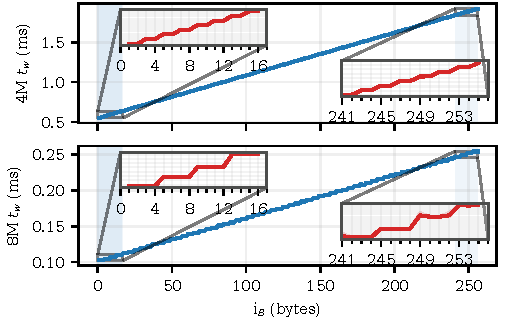
\includegraphics[width=0.95\linewidth]{fig/images/pdf/redundant-bytes-lineplots.pdf}
    \vspace{-.45cm}
    \caption{Write latency measurements ($t_w$) for $i$-byte redundant write operations on 4M (top) and 8M (bottom) devices.}
    % \vspace{-.65cm}
    % The aggregated redundant write times of four MB85AS4MT and four MB85AS8MT. All bursts are measured 10 times at 10 random 256B base addresses on each chip. All initial buffer data is randomized\, and each burst amount overwrites data redundantly from the base address up to the burst amount.}
    \label{fig:red-scan}
\end{figure}

\ssubsubsection{\textbf{Expt.~II 1-bit Transitions, Uniform $\mathrm{S}$}}
%\ssubsection*{Expt.~II Locally Uniform 1-bit Transitions}
\label{exp:ii}
In this experiment, we characterize single-bit write latency in uniformly-initialized 256-byte segments ($S$).
Single-bit transitions may exhibit data-dependent $t_w$ if there are asymmetries in the switching dynamics of the ReRAM cells and/or the PV loop.

% \begin{algorithm}[t]
\footnotesize
\caption{1-bit, uniform $\mathrm{S}$, test pattern generation \label{alg:1bit}}
\begin{algorithmic}[1]
\State $N_{\text{ADDRS}} \gets 10$
\State $A \gets$ rand\_256B\_aligned\_addrs($N_{\text{ADDRS}}$)
\ForAll{address \textbf{ in } $A$}
    \ForAll{$\mathrm{S}$ \textbf{ in } [$\mathbf{0}$, $\mathbf{1}$]}
        \State init\_$\mathrm{S}$(address, $\mathrm{S}$) \Comment{1, 256-byte write op}
        \State $L \gets$ shuffle(range(0, 2047))
        \ForAll{$i_{\text{b}}$ \textbf{ in } $L$}
            \State toggle\_bit\_i\_twice($\mathrm{S}$, $i_{\text{b}}$) 
            \Comment{2, 1-byte write ops}
        \EndFor
    \EndFor
\EndFor
\end{algorithmic}
\end{algorithm}



A 256-byte span ($\mathrm{S}$) is initialized to $\mathrm{S}=\mathbf{0}$ (all zeros)  or $\mathrm{S}=\mathbf{1}$  (all ones). Each bit positions ($i_b$) in the 2048-bit span is toggled 10 times and write latencies are captured. Since the minimum write size in both memories is 1 byte, we calculate the byte-offset and target data bit from $i_b$ and perform two 1-byte write latency measurements, toggling bit $i_b$ in both logical polarities.


Figure~\ref{fig:1b-buff-scan} demonstrates $t_w$ distributions for each chip.
Each bar in Figure~\ref{fig:1b-buff-scan} represents a log-scaled collapsed histogram, combining all bit positions and experiment addresses for one polarity, initial uniform state, and chip. 
Because the distributions are long-tailed, we truncate the plot at the 95th percentile to improve visibility.

The measured write latency distributions for each polarity measured from the 4M subtly overlap but are distinguishable. For the 8M, write latency distributions for each polarity are separated by a large margin. These write latency polarity relationships are preserved across all MB85AS4MT and MB85AS8MT samples. This experiment demonstrates that single-bit transitions of each memory produce data dependent write latency distributions.

\begin{figure}[h!]
    \centering
    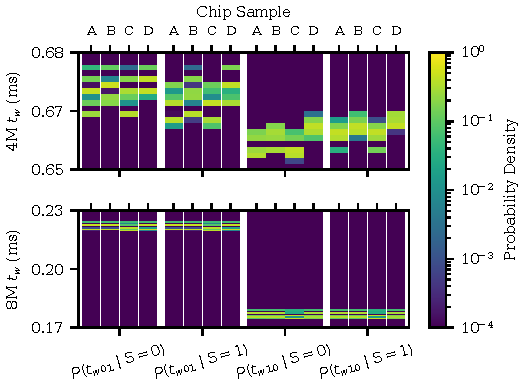
\includegraphics[width=0.95\linewidth]{fig/images/pdf/single-bit-buffer-scans-heat-bars.pdf}
    \vspace{-.5cm}
    \caption{Write latency distributions for 1-bit transitions within uniformly initialized 256-byte segments measured on 4 4M samples (top) and 4 8M samples (bottom). Each heatmap bar is a collapsed histogram colored according to the log-probability of observing a $t_w$ in each $\Delta t$-sized bin. $t_{w01}$ and $t_{w10}$ latencies correspond to data word transitions with a DHD of $\left(1,0 \right)$ and $\left(0,1\right)$, respectively. \label{fig:1b-buff-scan}}
\end{figure}
\begin{figure}[!h]
    \centering
    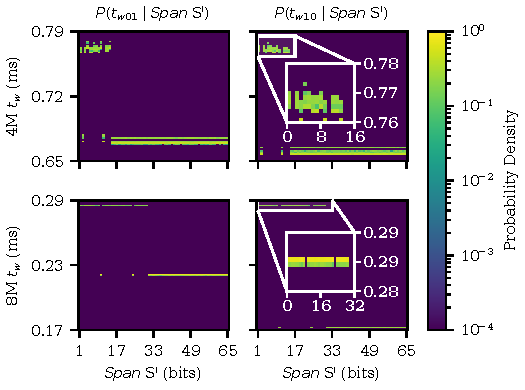
\includegraphics[width=0.95\linewidth]{fig/images/pdf/single-bit-sensitivity-scans-heat-bars-inset.pdf}
    \vspace{-.4cm}
    \caption{Write latency distributions for 1-bit $t_{w01}$ (left) and $t_{w10}$ (right) transitions within non-uniformly initialized 256-byte segments. Measurements from all 4 4M samples (top) and 4 8M samples (bottom) are aggregated. Each heatmap bar is a collapsed histogram colored according to the log-probability of observing a $t_w$ in each $\Delta t$-sized bin. The right plots zoom into the upper $t_w$ distributions to show 1-bit transitions that become \texttt{BIPOLAR} due to parity bit activity. \label{fig:sensitivity-scan}}
\end{figure}

\ssubsubsection{\textbf{Expt.~III 1-bit Transitions, Nonuniform $\mathrm{S}$}}
% \ssubsection*{Expt.~III Locally non-uniform 1-bit transitions}
\label{exp:iii}

% \begin{algorithm}[b!]
\footnotesize
\caption{1-bit, non-uniform $\mathrm{S}$, test pattern generation \label{alg:sensitivity}}
\begin{algorithmic}[1]
\State $N_{\text{ADDRS}} \gets 10$
\State $A \gets$ rand\_sample(align\_256B(addresses), $N_{\text{ADDRS}}$)
\State $\mathrm{S} \gets \mathbf{0}$
\ForAll{address \textbf{ in } $A$}
    \State $L \gets$ shuffle(range(1, 2047))
    \ForAll{$s$ \textbf{ in } $L$}
        \State $\mathrm{S}' \gets$ initialize\_$\mathrm{S}'$($\mathrm{S}$, $s$) \Comment{1, 256-byte write op}
        \State toggle\_bit\_0\_twice($\mathrm{S}'$) \Comment{2, 1-byte write ops}
    \EndFor
\EndFor
\end{algorithmic}
\end{algorithm}

ECC parity bit transition polarities depend on the state of a data word ($d$). In this experiment, we demonstrate that the state of non-transitioning bits can influence the $t_w$ distribution, indicating the presence of parity bits. By making $S$ non-uniform in the same word boundary as a transitioning bit, we demonstrate three distinct latency distributions. 
%In the next experiment, we demonstrate that these distributions correspond to the $\texttt{UNIPOLAR}_N$, $\texttt{UNIPOLAR}_P$, and \texttt{BIPOLAR} transitions in Table \ref{tab:polarity-mix}.

We randomly select 10 256-byte-aligned addresses. From each address, a 256-byte segment is initialized to all zeros ($\mathrm{S}=\mathbf{0}$).  
The first bit in each segment is designated as the \emph{measurement bit}.  
Before each measurement sequence, a contiguous subset of neighboring bits extending from the measurement bit is inverted ($\mathrm{S}[1:i] = \mathrm{S}' = \mathbf{1}$), creating a locally non-uniform initial state.  
Each measurement bit is toggled 10 times per configuration, with $\mathrm{S}'$ span sizes ($i$) ranging from 1 to 2047 bits.



The resulting distributions are shown in Figure~\ref{fig:sensitivity-scan}, with $\mathrm{S}'$ span sizes from 1-64. We make two key observations. First, beyond the word size reported in \hyperref[exp:i]{Exp.~I}, the distribution of write times stabilizes.
That is, the influence of nearby bit-states on write latency ends at the logical word boundary.  
Once the $\mathrm{S}'$ span exceeds the word length ($k$), the measured write latency distribution is identical to our prior, uniform $\mathrm{S}$, experiment.
Second, while the span of $\mathrm{S}'$ is smaller than the word boundary, single-bit writes generally exhibit longer latencies than those observed in uniform segments.
%In Section~\ref{}, we demonstrate that these high latency distributions are identical to those occupied by bipolar transitions.

% This effect is observed for both write polarities, and can be explained by non-uniform data causing parity bit activity in the opposing polarity to the measurement bit.  
% However, in both the MB85AS4MT and MB85AS8MT, two specific $\mathrm{S}'$ span configurations yield latency distributions nearly identical to those of the uniform baseline. These anomalies can be explained as data word configurations that result in consistent data and parity bit transition polarities.

% In summary, 1-bit write transitions demonstrate that the write polarity can be identified from uniformly initialized word boundaries. Additionally, the latency of 1-bit transitions is sensitive to the logical state of other bits within the same word. In the next experiment, we demonstrate that the highest write-latency cluster observed in \hyperref[exp:iii]{Exp. III} is the same latency cluster observed when measuring multi-bit bipolar byte transitions.

\ssubsubsection{\textbf{Expt.~IV 1-byte Transitions, Uniform $S$}}
\label{sec:1byte}
\label{exp:iv}
% We now characterize $t_w$ for all single-byte transitions on the MB85AS4MT and MB85AS8MT devices. The purpose of the following experiment is to identify the write latency properties of multi-bit transitions occurring within word boundaries. From our results, we are able to link $t_w$ timing cluster membership to unipolar and bipolar transitions.
% \paragraph*{\textbf{Exp.~IV 1-byte transitions}} 
In this experiment, we measure $t_w$ for all possible ($2^{16}$) single-byte transitions for all 4M and 8M samples.
This experiment is similar to the 1-byte latency characterization performed in \cite{tolga2024trng} where the 4M device was evaluated as an entropy source for true random number generators (TRNGs). We repeat the same experiment here. For each chip, the experiment is performed on 10 word-sized segments. We vary the state of all inactive bytes in the word, setting them to either all 1's or all 0's, and repeat our measurements for all bytes within each target segment. For each chip, to suppress the effect or rare long-tailed latency measurements, we take the minimum $t_w$ ($t_{wmin}$) for each byte transition across all segments.

Figure \ref{fig:sierp-hist} shows the results of this experiment for the 4M and 8M. We observe 3 unique $t_w$ distributions for the 4M chip, and 4 for the 8M chip. The minimum $t_w$ measurement distribution is exclusively occupied by redundant write operations. Bipolar dataword transitions always occupy the highest $t_w$ distribution. Unipolar dataword transitions occupy either a intermediate $t_w$ distribution or the highest $t_w$ distribution. For the 4M, unipolar dataword transitions occupying the intermediate $t_w$ distribution overlap. For the 8M, there are two distinct intermediate $t_w$ distributions, each occupied by $t_w$ measurements of a single datword transition polarity. These timing observations are consistent with \cite{tolga2024trng}. Our observation that certain \texttt{UNIPOLAR} transitions occupy \texttt{BIPOLAR} timing distributions suggests that underlying parity bit activity impacts the DHD of the write, causing polarity serialization.

% Considering the word boundaries identified Section \ref{sec:prelim-expts}, we expand this experiment to include all 2 (4) byte positions for each 2-byte (4-byte) word boundary within the MB85AS4MT (MB85AS8MT).
% \paragraph*{\textbf{Exp.~IV 1-byte transitions within 1-word writes}} 
% For each chip, we measure all byte transition $t_w$ for all byte positions of 10 word-sized segments ($\mathrm{S}$) where each word is initialized to either $\mathrm{S}=\mathbf{1}$ or $\mathrm{S}=\mathbf{0}$. Because our $t_w$ distributions are asymmetric and contain rare extreme-latency measurements, we use the per-chip minimum across all segments for each byte index and transition. This allows us to ensure these measurements do not impair our ability to distinguish the appropriate write latency distribution for each $t_w$.
% Test patterns are generated using Algorithm \ref{alg:1byte}. 
% We observe the same Sierpinski pattern as \cite{tolga2024trng} when our 4M measurements are visualized as a heatmap. We show our results as a histogram so that we can describe data-dependent polarity relationships for both the 4M and 8M in greater detail. 

% We assume that our $t_w$ measurement distributions map to the transition behavior of full codewords. In this context, parity bit activity cannot force a bipolar data word transition to produce a unipolar $t_w$, but it can cause a unipolar data word transition to occupy a bipolar $t_w$ if any parity bits transition toward an opposing polarity. If parity bits do not toggle or toggle only in a direction consistent with the applied data word transition, then the parity bits have no effect on the distribution that the resulting $t_w$ occupies. We identify each $t_{wmin}$ distribution using a parametric mixture model and label each mixture component shown in Figure \ref{fig:sierp-hist} with our inferred codeword behavior.

% The two initial states are used to confirm our prior finding that the state of the other bytes in the word effect the latencies of each byte under test. We note that similar analyses and visualization techniques as we present below have been performed on the MB85AS4MT device in \cite{tolga2024trng}, although this investigation did not consider the state of the other bytes in the word.
% To capture all 1-byte transition times we generate test patterns using Algorithm \ref{alg:1byte}. 
% % Note that each byte-transition is performed by writing an entire word. 
% % We choose to commit an entire word (where only 1 byte is active) for post-processing convenience and to maintain a similar data pattern between this experiment and the final one used for our SAT constraint encoding in Section \ref{sec:sat-encoding}.
% % \FloatBarrier
% \begin{algorithm}[!t]
\footnotesize
\caption{1-byte test pattern generation \label{alg:1byte}}
\begin{algorithmic}[1]
\State $B \gets$ word\_bytes() \Comment{2 for 4Mb, 4 for 8Mb}
\State $N_{\text{WORDS}} \gets 10$
\State $W \gets$ rand\_word\_aligned\_addrs($B$, $N_{\text{WORDS}}$)
\ForAll{word\_addr \textbf{ in } $W$}
    \ForAll{$G$ \textbf{ in } [$\mathbf{0}$, $\mathbf{1}$]}
        \State init\_word(word\_addr, $G$) \Comment{1, $B$-byte write op}
        \State $P \gets$ shuffle(range(0, $B{-}1$))
        \ForAll{byte\_pos \textbf{in} $P$}
            \State $Tr \gets$ get\_all\_byte\_transitions\_rand\_order()
            % \State from\_byte $\gets$ pack\_byte(byte\_pos, Tr[0].from)
            \State from\_byte $\gets$ Tr[0].from
            \State write\_byte(word\_addr, from\_byte)
            \Comment{1, 1-byte write op}
            \ForAll{tr \textbf{in} $Tr$}
                \State to\_byte $\gets$ tr.to
                \State write\_byte(word\_addr, to\_byte)
                \Comment{1, 1-byte write op}
            \EndFor
        \EndFor
    \EndFor
\EndFor
\end{algorithmic}
\end{algorithm}

\begin{figure}[t!]
    \centering
    \hspace{-0.75cm}
    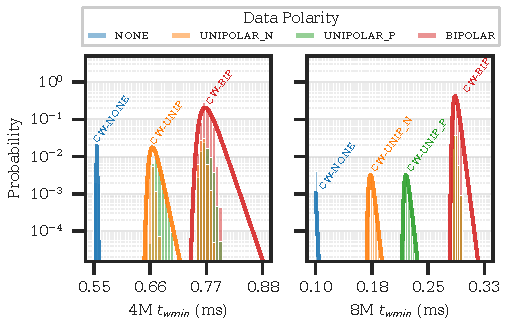
\includegraphics[width=0.95\columnwidth]{fig/images/pdf/sierpinski-clustering-mixture-curves.pdf}
    \vspace{-.45cm}
    \caption{4Mb and 8Mb $t_{wmin}$ measured for all 1-byte transitions. Histogram bars are colored according to data polarity. The curves correspond to EM-fitted mixture components that trace our observed latency clusters. We label each component according to our inferred codeword behavior \label{fig:sierp-hist}.}
    % \vspace{-.65cm}
\end{figure}
% % \FloatBarrier
% The results of our single-byte experiments are shown to the right in Figure \ref{fig:1B-sierpinski-scan}. We represent all transition times as pixels in a heatmap. For each heatmap, the x-axis is the initial state (FROM byte) of the transitioning byte in the word and the y-axis is it's final state (TO byte). 
% For this experiment, we take the minima of each per-chip write-latency distribution for each (TO, FROM) pair ($\min\left(t_{w}\right)$), to ensure long-tail write latencies do not bias aggregate statistics. We then average $\min\left(t_{w}\right)$ across all samples of each memory. We include two byte positions for each global setting. 

% As first identified in \cite{tolga2024trng}, a Sierpinski-like relationship with a minor hamming weight bias exists between all 1-byte transition test patterns and measured write latency. On the left of Figure \ref{fig:1B-sierpinski-scan}, a reference Sierpinski gasket is shown with a hamming weight bias. This image is generated by coloring points in the transition map where unipolar byte transitions occur. We also apply a small bias scaled to the total hamming weight of each transition to produce a close approximation of the measured heatmaps. Our measurements show three significant timing clusters (colors) for each heatmap. The fastest write latency group (black), always corresponds to redundant 1-byte write operations. The second fastest group (teal/blue) always corresponds 1-byte write operations with unipolar transitions. However, the slowest timing group (green/yellow) contains 1-byte write operations with both unipolar and bipolar transitions, puncturing the perfect Sierpinski gasket. Here we define a \textit{puncture} as a unipolar data-word transition whose write latency is similar to bipolar data word transitions. 

% Both bipolar and \emph{punctured} unipolar writes result in a similar $t_w$ as the long 1-bit writes observed under non-uniform initialization in the prior experiment.

% These results are consistent with the presence of a latent function that forces seemingly unipolar transitions (e.g. 1-bit transitions, unipolar byte transitions) to produce a bipolar write latency behavior. Within a crossbar memory, ECC is the most likely cause of this behavior. ECC parity bit states depend on the state of the data word. As parity bits are generally produced by XOR functions, when all but one bit in a data word is zero the transitioning bit is passed through. 

% In this case, if the parity matrix (P) produces parity bit transitioning in a direction oposing unipolar write data, this contradiction is expected.
% % out prior result where distribution shifts were observed for single-bit transitions, where the state of other bits in the word were changed ahead of transition measurements. 
% % From our \hyperref[exp:2ii]{Exp.~III} results, we found that there is a coupling between word-level bit states and write transition time. This results of this experiment demonstrates that the same coupling influences multi-bit transitions and that the timing cluster assignment of each transition is, for the most part, polarity dependent, and only violated when a unipolar data word results in bipolar timing. This effect suggests the presence of an ECC in our target memories. 
% As described in Section \ref{sec:bg}, ECC parity functions couple data bits to parity bits which are encoded and written in parallel with data bits. If parity bits update in a polarity opposing a unipolar data word transition, then the effective polarity (i.e. the polarity of the codeword transition) becomes bipolar. If they do not, then the entire codeword has a consistent polarity and the transition is unipolar. Bipolar transitions remain bipolar, independent of parity bit updates. This behavior perfectly describes our observations above. However, without the exact parity matrix, we cannot predict where parity bit perturbations will cause write latencies to diverge from the expected. In the next section we describe how BREW-RC capitalizes on this timing relationship to extract a bit-exact parity matrix from timing-polarity relationships.

\label{sec:clustering}

%\ssection{Experimental Setup}
The experiments described in the Sections \ref{sec:prelim-expts} and \ref{sec:brew-rc} are performed on four samples of two ReRAM products from RAMXeed. Specifications of interest for each device are listed in Table \ref{tab:reram_spec}.
Each experiment collects write latencies measuring the time to complete write operations, producing a dataset of write latencies corresponding to applied test vectors.
% \begin{equation}
% \mathcal{D} = \left(d_0^{(i)}, d_1^{(i)}, t_w^{(i)} \right)
% \end{equation}
% where $t_w^{(i)}$ is the measured write latency for the $i^{th}$ write operation transitioning an $n$-bit logically contiguous region from an initial state $d_0^{(i)} \in \left\{ 0,1\right\}^n$ to a final state
% $d_1^{(i)} \in \left\{ 0,1\right\}^n$.
Each write is committed to the memory over a SPI interface by de-asserting chip-select following the last byte of a $\texttt{WRITE}$ operation. Write latency is measured from the time the write transaction is committed, to the time the write-in-progress (WIP) bit of the STATUS register is cleared. Measurements of $t_w$ are quantized by the time required to check for the completion of a write ($\Delta t$). 
% Therefore, each write latency measurement is defined as
% \begin{equation}
% t_w \in \left\{i \Delta t \mid i \in \mathbb{N} \right\}
% \end{equation}
% where $i$ is the number of checks performed before for the $i^{th}$ write operation completes. 
$\Delta t$ is the minimum time required to perform a read status register (RDSR) operation on each RAMXeed module. The RDSR can be polled by continuing to drive the SPI clock after an initial opcode, returning the status after every 8 SPI cycles.
% The RDSR operation is required to determine when a committed write to memory completes. To perform a RDSR operation, the SPI bus must drive an initial 8-bit opcode followed by at least 8 SPI clock cycles to return the 8-bit status. After obtaining the first status byte, RDSR can continue to be polled by holding chip select while driving SPI clocks. In this polling mode, the status is returned every 8 SPI clock cycles (ignoring the initial opcode). 
The write completes when the write-in-progress (WIP) bit of the status register is cleared, and the write latency is recorded. The sampling period for measurements of $t_w$ is defined as the time between successive RDSR operations
$$ \Delta t = \frac{8}{f_{SPI}}.$$
We operate the SPI interfaces at the maximum frequency defined in the specification. Therefore, the minimum $\Delta t$ of the MB85AS4MT and MB85AS8MT memories are 1.6$\mu$s and 0.8$\mu$s, respectively.
%For any measurement of $t_w$, $\hat{t_w}$,  $t_w$ is at most $\hat{t_w}$ and at least $\hat{t_w} + T_{sample}$. In the write latency distributions presented in the rest of the paper, each measured $t_w$ is therefore quantized as
% \begin{equation}
% t_{k-1} \; T_{sample} < t_w \le t_k \; T_{sample} \implies \widehat{t}_w=t_k
% \end{equation}
We apply and time SPI transactions to all samples of the MB85AS4MT and MB85AS8MT ReRAM chips using a Terasic DE10-Nano Cyclone V SoC FPGA development kit. For each write operation, a counter on the FPGA captures $t_w$, which is then pushed to a response FIFO. The FPGA is used primarily to scale our experiments to many chips. Prior works have demonstrated similar timing capabilities using microcontrollers \cite{tolga2024trng, ferdaus2024hiding}.

\begin{table}[t!]
	\centering
	\caption{RAMXeed ReRAM device comparison.}
	\label{tab:reram_spec}
	\renewcommand{\arraystretch}{1.0}
	\setlength{\tabcolsep}{3.5pt}
	\begin{minipage}{0.98\columnwidth}
		\centering
		\begin{tabular}{lcccc}
			\toprule
			\textbf{Device}    & \textbf{Capacity}  & \textbf{SPI} $\mathbf{f_{\max}}$ &
			\textbf{Endurance} & \textbf{Buf. Size}                                                              \\
			\midrule
			\textbf{MB85AS4MT} & 4\,Mb              & 5\,MHz                           & 1.2M\,Times/B  & 256\,B \\
			\textbf{MB85AS8MT} & 8\,Mb              & 10\,MHz                          & 1M\,Times/4\,B & 256\,B \\
			\bottomrule
		\end{tabular}
	\end{minipage}
	% \vspace{-.5cm}
\end{table}



%\ssection{Preliminary Experiments}
\label{sec:prelim-expts}

We now present the timing side-channel enabling BREW-RC through a series of experiments performed on the MB85AS4MT (4M) and MB85AS8MT (8M) devices. 
Each experiment produces a set of write latency measurements corresponding to a test sequence. Measurements are carried out on 4 samples of each device.

\ssubsection*{Expt.~I Redundant-Write Write Latency}
%\ssubsection*{Expt.~I Redundant Writes}
\label{sec:red}
\label{exp:i}

% \begin{algorithm}[b]
\footnotesize
\caption{redundant write test pattern generation \label{alg:red}}
\begin{algorithmic}[1]
\State $N_{\text{ADDRS}} \gets 10$
\State $A \gets$ rand\_256B\_aligned\_addrs($N_{\text{ADDRS}}$)
\ForAll{address \textbf{ in } $A$}
    \State $\mathrm{S} \gets$ get\_rand\_256B\_pattern() 
    \State $L \gets$ shuffle(range(1, 256))
    \State write\_$\mathrm{S}$(address, $\mathrm{S}$) \Comment{1, 256-byte write op}
    \ForAll{$i$ \textbf{ in } $L$}
        \State write\_bytes(address, $\mathrm{S}[0{:}i]$) 
        \Comment{1, $i$-byte write op}
    \EndFor
\EndFor
\end{algorithmic}
\end{algorithm}
\begin{figure}[t!]
    \centering
    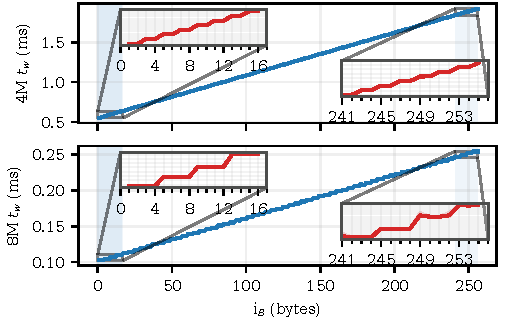
\includegraphics[width=0.95\linewidth]{fig/images/pdf/redundant-bytes-lineplots.pdf}
    \vspace{-.45cm}
    \caption{Write latency measurements ($t_w$) for $i$-byte redundant write operations on 4M (top) and 8M (bottom) devices.}
    % \vspace{-.65cm}
    % The aggregated redundant write times of four MB85AS4MT and four MB85AS8MT. All bursts are measured 10 times at 10 random 256B base addresses on each chip. All initial buffer data is randomized\, and each burst amount overwrites data redundantly from the base address up to the burst amount.}
    \label{fig:red-scan}
\end{figure}

In a crossbar-based architecture, the word size of the memory array is the smallest unit that can be serialized through the write path. Additionally, the word size is the natural choice for the ECC encoder data word width ($k$). Our target memories allow 1-256B write operations. However the physical word size of our target devices is not explicitly mentioned in the datasheets.

To infer $k$, we use the latency characteristics of redundant write operations. A \textit{redundant write} reinforces the existing logical state of ReRAM cells.  Because no transitions occur, the write latency reflects the minimum $t_{w}$ (Table \ref{tab:polarity-mix}) and the fixed per-word programming overhead of the controller. This makes redundant writes a low noise probe of the write-path serialization granularity. 

To determine $k$, we perform redundant writes with burst sizes of 1-256B on 10 randomly selected 256B-aligned addresses. First, we program a 256B contiguous memory segment ($\mathrm{S}$) to a random initial state. Then, for each byte position $i_B$ within ($\mathrm{S}$), an $i_B$-byte redundant write is performed.

Figure \ref{fig:red-scan} shows the combined write latencies (mean and shaded 95\% confidence interval) for all samples and test addresses. For each 4M (8M) sample, at all addresses, and across all randomly initialized $S$ states, $t_w$ overheads are accrued every two (four) byte-lengths and show almost no variance. This result demonstrates that 4M (8M) redundant write times do not show a clear data dependency, and that serialization occurs on 2B (4B) boundaries, indicating $k_{4M}=16$ bits ($k_{8M}=32$ bits). We will use $k_{4M}$ and $k_{8M}$ to constrain one dimension our parity submatrix in Section \ref{fig:brew-rc}.

\ssubsection*{Expt.~II 1-bit Transitions, Uniform $\mathrm{S}$}
%\ssubsection*{Expt.~II Locally Uniform 1-bit Transitions}
\label{exp:ii}
Single-bit transitions may exhibit data-dependent $t_w$ if there are asymmetries in the switching dynamics of the ReRAM cells and/or the PV loop. In this experiment, we characterize single-bit write latency in uniformly initialized 256-byte segments ($S$), where all non-transitioning bits are initialized to a uniform logical state.

% \begin{algorithm}[t]
\footnotesize
\caption{1-bit, uniform $\mathrm{S}$, test pattern generation \label{alg:1bit}}
\begin{algorithmic}[1]
\State $N_{\text{ADDRS}} \gets 10$
\State $A \gets$ rand\_256B\_aligned\_addrs($N_{\text{ADDRS}}$)
\ForAll{address \textbf{ in } $A$}
    \ForAll{$\mathrm{S}$ \textbf{ in } [$\mathbf{0}$, $\mathbf{1}$]}
        \State init\_$\mathrm{S}$(address, $\mathrm{S}$) \Comment{1, 256-byte write op}
        \State $L \gets$ shuffle(range(0, 2047))
        \ForAll{$i_{\text{b}}$ \textbf{ in } $L$}
            \State toggle\_bit\_i\_twice($\mathrm{S}$, $i_{\text{b}}$) 
            \Comment{2, 1-byte write ops}
        \EndFor
    \EndFor
\EndFor
\end{algorithmic}
\end{algorithm}

\begin{figure}[h!]
    \centering
    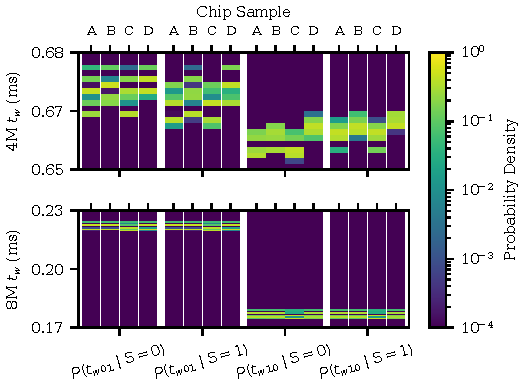
\includegraphics[width=0.95\linewidth]{fig/images/pdf/single-bit-buffer-scans-heat-bars.pdf}
    \vspace{-.5cm}
    \caption{Write latency distributions for 1-bit transitions within uniformly initialized 256-byte segments measured on 4 4M samples (top) and 4 8M samples (bottom). Each heatmap bar is a collapsed histogram colored according to the log-probability of observing a $t_w$ in each $\Delta t$-sized bin. $t_{w01}$ and $t_{w10}$ latencies correspond to data word transitions with a DHD of $\left(1,0 \right)$ and $\left(0,1\right)$, respectively. \label{fig:1b-buff-scan}}
\end{figure}

At each address, a contiguous 256-byte span ($\mathrm{S}$) is initialized to $\mathrm{S}=\mathbf{0}$ (all zeros)  or $\mathrm{S}=\mathbf{1}$  (all ones). Each bit positions ($i_b$) in the 2048-bit span is toggled 10 times and write latencies are captured. The minimum write size in both memories is 1 byte. Therefore we calculate the byte-offset and target data bit from $i_b$ and perform two 1-byte write latency measurements, toggling bit $i_b$ in both logical polarities.
The resulting $t_w$ measurement distributions for each chip are shown in Figure~\ref{fig:1b-buff-scan}.
Each bar in Figure~\ref{fig:1b-buff-scan} represents a log-scaled collapsed histogram, combining all bit positions and experiment addresses for one polarity, initial uniform state, and chip. 
Because the distributions are long-tailed, we truncate the plot at the 95th percentile to improve visibility.

The measured write latency distributions for each polarity measured from the 4M subtly overlap but are distinguishable. For the 8M, write latency distributions for each polarity are separated by a large margin. These write latency polarity relationships are preserved across all MB85AS4MT and MB85AS8MT samples. This experiment demonstrates that single-bit transitions of each memory produce data dependent write latency distributions.

\ssubsection*{Expt.~III 1-bit Transitions, Nonuniform $\mathrm{S}$}
% \ssubsection*{Expt.~III Locally non-uniform 1-bit transitions}
\label{exp:iii}

% \begin{algorithm}[b!]
\footnotesize
\caption{1-bit, non-uniform $\mathrm{S}$, test pattern generation \label{alg:sensitivity}}
\begin{algorithmic}[1]
\State $N_{\text{ADDRS}} \gets 10$
\State $A \gets$ rand\_sample(align\_256B(addresses), $N_{\text{ADDRS}}$)
\State $\mathrm{S} \gets \mathbf{0}$
\ForAll{address \textbf{ in } $A$}
    \State $L \gets$ shuffle(range(1, 2047))
    \ForAll{$s$ \textbf{ in } $L$}
        \State $\mathrm{S}' \gets$ initialize\_$\mathrm{S}'$($\mathrm{S}$, $s$) \Comment{1, 256-byte write op}
        \State toggle\_bit\_0\_twice($\mathrm{S}'$) \Comment{2, 1-byte write ops}
    \EndFor
\EndFor
\end{algorithmic}
\end{algorithm}
\begin{figure}[!h]
    \centering
    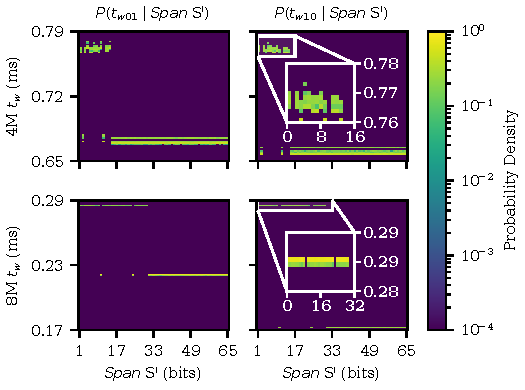
\includegraphics[width=0.95\linewidth]{fig/images/pdf/single-bit-sensitivity-scans-heat-bars-inset.pdf}
    \vspace{-.4cm}
    \caption{Write latency distributions for 1-bit $t_{w01}$ (left) and $t_{w10}$ (right) transitions within non-uniformly initialized 256-byte segments. Measurements from all 4 4M samples (top) and 4 8M samples (bottom) are aggregated. Each heatmap bar is a collapsed histogram colored according to the log-probability of observing a $t_w$ in each $\Delta t$-sized bin. The right plots zoom into the upper $t_w$ distributions to show 1-bit transitions that become \texttt{BIPOLAR} due to parity bit activity. \label{fig:sensitivity-scan}}
\end{figure}

ECC parity bit transition polarities depend on the state of a data word ($d$). In this experiment, we demonstrate that the state of non-transitioning bits can influence the $t_w$ distribution, indicating the presence of parity bits. By making $S$ non-uniform in the same word boundary as a transitioning bit, we demonstrate that three distinct latency distribution emerge. In the next experiment, we demonstrate that these distributions correspond to the $\texttt{UNIPOLAR}_N$, $\texttt{UNIPOLAR}_P$, and \texttt{BIPOLAR} transitions in Table \ref{tab:polarity-mix}.

10 256-byte-aligned addresses are randomly selected. From each address, a 256-byte span is initialized to all zeros ($G=\mathbf{0}$).  
The first bit in each segment is designated as the \emph{measurement bit}.  
Before each measurement sequence, a contiguous subset of neighboring bits extending from the measurement bit is inverted ($\mathrm{S}[1:i] = \mathrm{S}' = \mathbf{1}$), creating a locally non-uniform initial state.  
Each measurement bit is toggled 10 times per configuration, with $\mathrm{S}'$ span sizes ($i$) ranging from 1 to 2047 bits.

The resulting distributions are shown in Figure~\ref{fig:sensitivity-scan} showing $\mathrm{S}'$ span sizes from 1-64. We now make two key observations. First, beyond the word size reported in \hyperref[exp:i]{Exp.~I}, the distribution of write times stabilize.
That is, the influence of nearby bit-states on write latency ends at the logical word boundary.  
Once the $\mathrm{S}'$ span exceeds the word length ($k$), the measured write latency distribution is identical to our prior, uniform $\mathrm{S}$, experiment.
Second, while the span of $\mathrm{S}'$ is smaller than the word boundary, single-bit writes generally exhibit substantially longer latencies than those observed in uniform segments. In the next section, we demonstrate that these high latency distributions are identical to those occupied by bipolar transitions.

% This effect is observed for both write polarities, and can be explained by non-uniform data causing parity bit activity in the opposing polarity to the measurement bit.  
% However, in both the MB85AS4MT and MB85AS8MT, two specific $\mathrm{S}'$ span configurations yield latency distributions nearly identical to those of the uniform baseline. These anomalies can be explained as data word configurations that result in consistent data and parity bit transition polarities.

% In summary, 1-bit write transitions demonstrate that the write polarity can be identified from uniformly initialized word boundaries. Additionally, the latency of 1-bit transitions is sensitive to the logical state of other bits within the same word. In the next experiment, we demonstrate that the highest write-latency cluster observed in \hyperref[exp:iii]{Exp. III} is the same latency cluster observed when measuring multi-bit bipolar byte transitions.

\ssubsection*{Expt.~IV 1-byte Transitions, Uniform $S$}

\label{sec:1byte}
\label{exp:iv}
% We now characterize $t_w$ for all single-byte transitions on the MB85AS4MT and MB85AS8MT devices. The purpose of the following experiment is to identify the write latency properties of multi-bit transitions occurring within word boundaries. From our results, we are able to link $t_w$ timing cluster membership to unipolar and bipolar transitions.

% \paragraph*{\textbf{Exp.~IV 1-byte transitions}} 
In this experiment, the latency properties of all possible ($2^{16}$) single byte transition $t_w$ are investigated.
This experiment is similar to the 1-byte latency characterization performed in \cite{tolga2024trng} where 4M device timing was evaluated as an entropy source for true random number generators (TRNGs). We repeat the same experiment here, however, we vary the state of all inactive bytes in the word, setting them to either all 1's or all 0's, to exercise the entire dataword. The authors of \cite{tolga2024trng} note that when the latency of each single-byte transition is visualized as a heatmap, a noisy Sierpinski-gasket pattern is generated. A perfect Sierpinski pattern can be drawn by coloring unipolar transitions, although the Sierpinski gasket generated in \cite{tolga2024trng} is punctured. This finding is consistent with our observations in \hyperref[exp:iii]{Exp.~III} that $t_w$ \emph{may be} minimized for some, but not all $\texttt{UNIPOLAR}$ transitions.
% Considering the word boundaries identified Section \ref{sec:prelim-expts}, we expand this experiment to include all 2 (4) byte positions for each 2-byte (4-byte) word boundary within the MB85AS4MT (MB85AS8MT).
% \paragraph*{\textbf{Exp.~IV 1-byte transitions within 1-word writes}} 
For each chip, we measure all byte transition $t_w$ for all byte positions of 10 word-sized segments ($\mathrm{S}$) where each word is initialized to either $\mathrm{S}=\mathbf{1}$ or $\mathrm{S}=\mathbf{0}$. Because our $t_w$ distributions are asymmetric and contain rare extreme-latency measurements, we use the per-chip minimum across all segments for each byte index and transition. This allows us to ensure these measurements do not impair our ability to distinguish the appropriate write latency distribution for each $t_w$.
% Test patterns are generated using Algorithm \ref{alg:1byte}. 

We observe the same Sierpinski pattern as \cite{tolga2024trng} when our 4M measurements are visualized as a heatmap. Instead of a heatmap, we show our results as a histogram so that we can describe data-dependent polarity relationships for both the 4M and 8M in greater detail. Figure \ref{fig:sierp-hist} shows the results of this experiment for the 4M and 8M. We observe 3 (4) unique $t_w$ distributions. The minimum $t_w$ measurement distribution is exclusively occupied by redundant write operations. Bipolar dataword transitions always occupy the highest $t_w$ distribution. Unipolar dataword transitions occupy either a moderate $t_w$ distribution or the highest $t_w$ distribution. For the 4M, unipolar dataword transitions occupying the moderate $t_w$ distribution overlap. For the 8M there are two distinct moderate $t_w$ distributions, each occupied by $t_w$ measurements of a single datword transition polarity. 

We assume that our $t_w$ measurement distributions map to the transition behavior of full codewords. In this context, parity bit activity cannot force a bipolar data word transition to produce a unipolar $t_w$, but it can cause a unipolar data word transition to occupy a bipolar $t_w$ if any parity bits transition toward an opposing polarity. If parity bits do not toggle or toggle only in a direction consistent with the applied data word transition, then the parity bits have no effect on the distribution that the resulting $t_w$ occupies. We cluster each $t_w$ distributions using a parametric mixture model and label each mixture component shown in Figure \ref{fig:sierp-hist} with our inferred codeword behavior.

% The two initial states are used to confirm our prior finding that the state of the other bytes in the word effect the latencies of each byte under test. We note that similar analyses and visualization techniques as we present below have been performed on the MB85AS4MT device in \cite{tolga2024trng}, although this investigation did not consider the state of the other bytes in the word.
% To capture all 1-byte transition times we generate test patterns using Algorithm \ref{alg:1byte}. 
% % Note that each byte-transition is performed by writing an entire word. 
% % We choose to commit an entire word (where only 1 byte is active) for post-processing convenience and to maintain a similar data pattern between this experiment and the final one used for our SAT constraint encoding in Section \ref{sec:sat-encoding}.
% % \FloatBarrier
% \begin{algorithm}[!t]
\footnotesize
\caption{1-byte test pattern generation \label{alg:1byte}}
\begin{algorithmic}[1]
\State $B \gets$ word\_bytes() \Comment{2 for 4Mb, 4 for 8Mb}
\State $N_{\text{WORDS}} \gets 10$
\State $W \gets$ rand\_word\_aligned\_addrs($B$, $N_{\text{WORDS}}$)
\ForAll{word\_addr \textbf{ in } $W$}
    \ForAll{$G$ \textbf{ in } [$\mathbf{0}$, $\mathbf{1}$]}
        \State init\_word(word\_addr, $G$) \Comment{1, $B$-byte write op}
        \State $P \gets$ shuffle(range(0, $B{-}1$))
        \ForAll{byte\_pos \textbf{in} $P$}
            \State $Tr \gets$ get\_all\_byte\_transitions\_rand\_order()
            % \State from\_byte $\gets$ pack\_byte(byte\_pos, Tr[0].from)
            \State from\_byte $\gets$ Tr[0].from
            \State write\_byte(word\_addr, from\_byte)
            \Comment{1, 1-byte write op}
            \ForAll{tr \textbf{in} $Tr$}
                \State to\_byte $\gets$ tr.to
                \State write\_byte(word\_addr, to\_byte)
                \Comment{1, 1-byte write op}
            \EndFor
        \EndFor
    \EndFor
\EndFor
\end{algorithmic}
\end{algorithm}

\begin{figure}[t!]
    \centering
    \hspace{-0.75cm}
    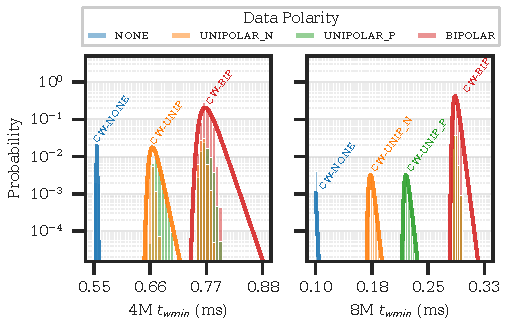
\includegraphics[width=0.95\columnwidth]{fig/images/pdf/sierpinski-clustering-mixture-curves.pdf}
    \vspace{-.45cm}
    \caption{4Mb and 8Mb $t_{wmin}$ measured for all 1-byte transitions. Histogram bars are colored according to data polarity. The curves correspond to EM-fitted mixture components that trace our observed latency clusters. We label each component according to our inferred codeword behavior \label{fig:sierp-hist}.}
    % \vspace{-.65cm}
\end{figure}
% % \FloatBarrier
% The results of our single-byte experiments are shown to the right in Figure \ref{fig:1B-sierpinski-scan}. We represent all transition times as pixels in a heatmap. For each heatmap, the x-axis is the initial state (FROM byte) of the transitioning byte in the word and the y-axis is it's final state (TO byte). 
% For this experiment, we take the minima of each per-chip write-latency distribution for each (TO, FROM) pair ($\min\left(t_{w}\right)$), to ensure long-tail write latencies do not bias aggregate statistics. We then average $\min\left(t_{w}\right)$ across all samples of each memory. We include two byte positions for each global setting. 

% As first identified in \cite{tolga2024trng}, a Sierpinski-like relationship with a minor hamming weight bias exists between all 1-byte transition test patterns and measured write latency. On the left of Figure \ref{fig:1B-sierpinski-scan}, a reference Sierpinski gasket is shown with a hamming weight bias. This image is generated by coloring points in the transition map where unipolar byte transitions occur. We also apply a small bias scaled to the total hamming weight of each transition to produce a close approximation of the measured heatmaps. Our measurements show three significant timing clusters (colors) for each heatmap. The fastest write latency group (black), always corresponds to redundant 1-byte write operations. The second fastest group (teal/blue) always corresponds 1-byte write operations with unipolar transitions. However, the slowest timing group (green/yellow) contains 1-byte write operations with both unipolar and bipolar transitions, puncturing the perfect Sierpinski gasket. Here we define a \textit{puncture} as a unipolar data-word transition whose write latency is similar to bipolar data word transitions. 

% Both bipolar and \emph{punctured} unipolar writes result in a similar $t_w$ as the long 1-bit writes observed under non-uniform initialization in the prior experiment.

% These results are consistent with the presence of a latent function that forces seemingly unipolar transitions (e.g. 1-bit transitions, unipolar byte transitions) to produce a bipolar write latency behavior. Within a crossbar memory, ECC is the most likely cause of this behavior. ECC parity bit states depend on the state of the data word. As parity bits are generally produced by XOR functions, when all but one bit in a data word is zero the transitioning bit is passed through. 

% In this case, if the parity matrix (P) produces parity bit transitioning in a direction oposing unipolar write data, this contradiction is expected.
% % out prior result where distribution shifts were observed for single-bit transitions, where the state of other bits in the word were changed ahead of transition measurements. 
% % From our \hyperref[exp:2ii]{Exp.~III} results, we found that there is a coupling between word-level bit states and write transition time. This results of this experiment demonstrates that the same coupling influences multi-bit transitions and that the timing cluster assignment of each transition is, for the most part, polarity dependent, and only violated when a unipolar data word results in bipolar timing. This effect suggests the presence of an ECC in our target memories. 
% As described in Section \ref{sec:bg}, ECC parity functions couple data bits to parity bits which are encoded and written in parallel with data bits. If parity bits update in a polarity opposing a unipolar data word transition, then the effective polarity (i.e. the polarity of the codeword transition) becomes bipolar. If they do not, then the entire codeword has a consistent polarity and the transition is unipolar. Bipolar transitions remain bipolar, independent of parity bit updates. This behavior perfectly describes our observations above. However, without the exact parity matrix, we cannot predict where parity bit perturbations will cause write latencies to diverge from the expected. In the next section we describe how BREW-RC capitalizes on this timing relationship to extract a bit-exact parity matrix from timing-polarity relationships.

\label{sec:clustering}
\ssection{BREW-RC}
\label{sec:brew-rc}
We now present our method for bit-exact recovery of ECC in ReRAM crossbars, BREW-RC.
% First, we relate the observed timing behavior—captured as data transitions and their clustering assignments to a latent model defined by an ECC parity matrix, which governs parity-bit switching under a linear block code (LBC).
% Next, we introduce a test-vector generation strategy that guarantees each write-latency measurement ($t_w$) produces a corresponding logical constraint. 
% Finally, we present the resulting SAT-based recovery results. In the following section, we use these results to interpret related work on the MB85AS4MT and MB85AS8MT memories.
% We note here that we must make an assumption that the latent behavior observed in our prior experiments is an ECC function. We admit that this assumption is slightly weaker than the one made in our motivating work \cite{patel2020bit}. In \cite{patel2020bit}, the authors test only modules that advertise ECC capabilities. The datasheet of both devices under test make no mention of error correcting codes, whereas this is common practice for DRAM modules. 
% Our interests, however, reside in the domain of hardware side-channels where an adversary's initial objective is to construct a model of an information leakage channel. Our motivation is therefore related to BEER but not identical.
% \ssubsection{Polarity Relationships and Measurement Pruning}
Section~\ref{sec:clustering} demonstrates that timing measurement distributions identify polarity relationships of entire codewords ($\{\texttt{NONE},\texttt{UNIPOLAR}, \texttt{BIPOLAR}\}$). These distributions are defined with labels:
{
\setlength{\abovedisplayskip}{1pt}
\setlength{\belowdisplayskip}{0.5pt}
\begin{equation}
\ell_{cw}, \ell_d \in \{\texttt{NONE}, \texttt{UNIPOLAR\_P}, \texttt{UNIPOLAR\_N}, \texttt{BIPOLAR}\}.
\end{equation}
} 
where the label ($\ell_{cw}$) reflects the codeword DHD and $\ell_d$ is the known transition polarity of the applied data. Note that a conversion from $\texttt{UNIPOLAR}$ observations to a corresponding $\texttt{UNIPOLAR\_P}$ / $ \texttt{UNIPOLAR\_N}$ label may be required (i.e. 4M, Figure \ref{fig:sierp-hist}). This is trivial as the transition polarity of a unipolar codeword must be identical to the transition polarity of the dataword. We describe the relationship between the applied data and codeword transition label with the shorthand $\ell_{d} \rightarrow\ell_{cw}$.

% Some transition relationships between known dataword DHD and observed codeword DHD derived from $t_w$ measurements are consistent
% (ex. $\texttt{NONE}$ $\rightarrow\texttt{NONE}$, $\texttt{BIPOLAR}\rightarrow\texttt{BIPOLAR}$,  $\texttt{UNIPOLAR}_{N/P}\rightarrow\texttt{UNIPOLAR}_{N/P}$). 
$\texttt{NONE}\rightarrow\texttt{NONE}$ transitions reveal nothing about the parity function. As we showed in Section \ref{sec:red}, the timing of these transitions is related to write serialization overhead and has almost zero variance. 
$\texttt{BIPOLAR}\rightarrow\texttt{BIPOLAR}$ also gives no information. These observations essentially translate to: ``given a forced \texttt{BIPOLAR} multi-bit data transition, the parity bits may or may not have transitioned in any polarity.''
Some observations would violate our hypothesis that parity bit polarity serialization is the cause of our observed timing fluctuations (ex. $\texttt{NONE} \to \texttt{UNIPOLAR}_{N/P}$,  $\texttt{BIPOLAR}\rightarrow\texttt{UNIPOLAR}_{N/P}$ ). We implement assertions to validate that they are never observed.

BREW-RC uses two observation classes to generate SAT constraints.
$\texttt{UNIPOLAR}_{N/P}\rightarrow\texttt{UNIPOLAR}_{N/P}$ reveal an explicit constraint: ``given a $\texttt{UNIPOLAR}_{N/P}$, data transition, no parity bits transition in an opposing polarity.'' $\texttt{UNIPOLAR}_{N/P}\rightarrow\texttt{BIPOLAR}$ produce an existential constraint that translates to: ``given a $\texttt{UNIPOLAR}_{N/P}$ data transition, at least one parity bit transitioned in an opposing polarity.''

\ssubsection{Modeling parity-bit activity}
As described in Section~\ref{sec:bg}, ReRAM memories often employ linear block codes (LBCs). For a dataword $d\in\{0,1\}^k$, the codeword $c=dG=[d\mid p]$ propagates data bits ($d$) and appends generated parity bits generated by the $GF(2)$ multiplication
{
\setlength{\abovedisplayskip}{1pt}
\setlength{\belowdisplayskip}{1pt}
\begin{equation}
    p = dP.
\end{equation}
}
For pre- and post-write states $(d_0,d_1)$, the parity-bit updates are
{
\setlength{\abovedisplayskip}{1pt}
\setlength{\belowdisplayskip}{1pt}
\begin{equation}
    \Delta p = (d_0 + d_1)P = \Delta d P,
\end{equation}
}
where $\Delta d=d_0+d_1$ marks toggled data bits.  
Thus, $\Delta p$ acts as a logical gate that determines which parity bits update under a given data transition, independent of transition polarity.  
In the SAT construction, $\Delta p$ is evaluated for every dataword transition and used in all clauses to restrict parity-bit activity to the toggled subset.

\ssubsection{Polarity-encoded SAT formulation}
\label{sec:sat-encoding}

To incorporate polarity, each transition is assigned a data-polarity label $\ell_d \in \{\texttt{UNIPOLAR\_P},\texttt{UNIPOLAR\_N}\}$ 
with scalar representation $d\in\{-1,+1\}$:
$d=+1$ for positive ($0{\rightarrow}1$) and $d=-1$ for negative ($1{\rightarrow}0$) unipolar transitions.
Bipolar and static cases (\texttt{BIPOLAR}, \texttt{NONE}) produce no directional information and are excluded.

For each parity bit $p_j$, Boolean variables $p_{0,j}$ and $p_{1,j}$ denote its pre- and post-write values, gated by $\Delta p_j$. 
We then define
{
\setlength{\abovedisplayskip}{1pt}
\setlength{\belowdisplayskip}{1pt}
\begin{align}
    \textit{pos}_j &\leftrightarrow \Delta p_j \wedge (\neg p_{0,j} \wedge p_{1,j}), \\
    \textit{neg}_j &\leftrightarrow \Delta p_j \wedge (p_{0,j} \wedge \neg p_{1,j}).
\end{align}
}
encoding positive and negative parity transitions only when the parity bit is expected to update.  
Depending on $(\ell_d,\ell_{cw})$, one of four clause types is generated as summarized in Table~\ref{tab:polarity-clauses}.  
Under unipolar test patterns, the \texttt{NONE} cluster is unobservable (more than zero bits are active). 
A \texttt{BIPOLAR} observation indicates that at least one parity bit transitioned in the opposite polarity to the data.
Conversely, a matching unipolar observation indicates the absence of any opposite-polarity parity transition.

Each $(d_0,d_1,\ell_d,\ell_{cw})$ tuple contributes a compact SAT subproblem constraining the allowed polarity of parity-bit transitions under a candidate parity submatrix ($P$).  

Because prior measurements exercised only single-bit or single-byte toggles, the resulting clauses may not reveal cross-byte parity coupling. Additionally, redundant writes and bipolar dataword transitions that are not useful, as they do not emit SAT constraints. Therefore, we introduce a \emph{unipolar random word walk} that systematically explores unipolar transitions over word regions, efficiently sampling the full word-level unipolar transition space.
\begin{table}[t!]
\setlength{\textfloatsep}{0pt}
\setlength{\floatsep}{0pt}
\centering
\caption{SAT solver clause definitions \label{tab:polarity-clauses}.}
\vspace{-.2cm}
\renewcommand{\arraystretch}{1.1}
\setlength{\tabcolsep}{3pt}
\begin{tabular*}{\linewidth}{@{\extracolsep{\fill}}lcccc@{}}
\toprule
\textbf{Data label} $\ell_d$ & \textbf{Obs.} $\ell_{cw}$ & \textbf{Constraint} & \textbf{Description} \\
\midrule
\texttt{UNIPOLAR\_P} & \texttt{UNIPOLAR\_P} & $\forall j\, (p_{0,j}\vee\neg p_{1,j})$  & forbid \emph{neg}  \\
\texttt{UNIPOLAR\_N} & \texttt{UNIPOLAR\_N} & $\forall j\, (\neg p_{0,j}\vee p_{1,j})$ & forbid \emph{pos} \\
\texttt{UNIPOLAR\_P} & \texttt{BIPOLAR}     & $\bigvee_j \textit{neg}_j$               & require $\ge1$ \emph{neg}  \\
\texttt{UNIPOLAR\_N} & \texttt{BIPOLAR}     & $\bigvee_j \textit{pos}_j$               & require $\ge1$ \emph{pos}  \\
\bottomrule
\end{tabular*}  
\end{table}
\setlength{\textfloatsep}{-10pt} {
	% \setlength{\floatsep}{-10pt}
	\begin{algorithm}[t!]
		\footnotesize
		\caption{1-word, random, unipolar walk\label{alg:ruw}}
		\begin{algorithmic}[1]
			\Require word size $k$, length $\ell$, max test-vectors per address $\textit{max\_tv}$
			\State $\texttt{Keys} \gets \varnothing$; $\texttt{A} \gets \varnothing$; \Comment{used transitions, used addrs.}
			\While{$i < \ell$}
			\If{$i \bmod \text{max\_tv} = 0$}
			\State $\texttt{addr}\gets\texttt{GetRandWordAddr(A)}$; $\texttt{A} \cup \texttt{addr}$;
			\State $s \gets \texttt{GetRandWord()}$;
			\State write\_word(addr, $s$)
			\EndIf
			\State $d \gets  s=0 \; ? \; 1 : s=2^k-1 \; ? \; 0 : \texttt{RNG(0,1)}))$;
			\State $m \gets \texttt{RNG(1, $2^k -1$)}$
			\State $s' \gets d=0\; ? \;s\; \& \; \neg m : s\; | \; m $;
			\State $key \gets \min(s,s') << k \; | \; max(s, s')$;
			\If{$\texttt{key} \notin \texttt{Keys}$}
			\State $\texttt{Keys} \cup \texttt{k}$ ; $s \gets s'$ ; $i\gets i+1$;
			\State write\_word($\texttt{addr}$, $s'$)
			\EndIf
			\EndWhile
		\end{algorithmic}
	\end{algorithm}
}
\setlength{\textfloatsep}{3pt}

\ssubsection{BREW-RC Data Collection}
\label{exp:2ii}
To ensure every test vector emits a useful constraint, we perform a random unipolar walk of the dataword space, and measure $t_{w}$ for every applied test vector. The details of this test-vector generation technique are shown in Alg. \ref{alg:ruw}. This procedure ensures that a unique unipolar dataword transition is generated for every write operation in the programming sequence.

% A random word-aligned address in memory is selected, and initialized to a random state. Then a direction (0 for \textit{neg}, 1 for \textit{pos}) is randomly selected. A random mask is generated according to the polarity, and then applied to the last test vector to generate the next unipolar random transition. This process repeats until the desired number of transitions have been applied. To ensure selected addresses are not worn out over the course of long experiments, we log wear levels and select new addresses once a threshold has been met. 

The 4M has a much higher probability of generating $\texttt{UNIPOLAR}_{P/N}$ $\to \texttt{UNIPOLAR}_{P/N}$ constraints due to it's significantly smaller parity submatrix than the 8M. For each chip, we repeat the experiment 10 times at different word addresses to generate a representative $t_{wmin}$. In order for BREW-RC to converge to a single ECC, we collect 100K (200K) $t_{wmin}$ from each 4M (8M) sample. 

After capturing timing data, we assign labels to construct $(d_0,d_1,$ $\ell_d,$ $\ell_{cw}$) observations. Each observation yields a set of XOR constraints encoding $\Delta p$ and CNF clauses enforcing the allowed polarity of each parity-bit transition. The resulting hybrid XOR+CNF formula is solved using CryptoMiniSAT \cite{soos2009extending, soos2018cryptominisat5}.

% Figure \ref{fig:1w-rand-walk} shows the distribution of $\min\left(t_{w}\right)$ measurements normalized for each chip along with the empirical cumulative distribution function. The upper plots show labels applied by clustering the $\min\left(t_{ws}\right)$ observations ($\ell_{cw}$), and the lower plots show labels applied using only the known data transitions ($\ell_d$). Clustering is performed using a mixture of extreme-value (Gumbel) distributions to capture the timing model discussed in \ref{sec:bg}.
% \begin{figure}[t!]
    \centering
    
\includegraphics[width=0.99\columnwidth]{fig/images/single-word-rand-walk-clustering.pdf}
    \Description{Histograms for the 4Mb and 8Mb write latencies measured for the random walk experiment are shown. The X-axis is the mix-max normalized write latency and the y-axis is the log-probability that a write latency is observed. Write latencies appear in three distinct distributions. Each distribution appears as a light-tailed left-skewed distribution. Histograms for \texttt{UNIPOLAR\_N}, \texttt{UNIPOLAR\_P} test vectors are overlaied and shown in different colors. The leftmost (slowest) distribution contains only \texttt{UNIPOLAR\_N}, the middle distribution contains mostly \texttt{UNIPOLAR\_P} (In the 4Mb it overlaps with  \texttt{UNIPOLAR\_N}), and the rightmost distribution for both memories contains a mixture of the two.}
    \caption{Per-chip min-max normalized $\min \left(t_{w}\right)$ measurement histograms and ECDFs for a 1-word random unipolar walk experiment used for BREW-RC constraint generation. Clustering is performed per-chip to demonstrate reproducibility across samples. Labels are assigned either naively from applied test vector data (bottom), or from clustering performed on observed write latencies (top). \label{fig:1w-rand-walk}}
\end{figure}
% To adequately exercise the ECC function, such that we can recover a single ECC function up to column permutations, we require test vectors that exercise all possible intra-bit coupling. We implement a simple unipolar random walk test vector generator shown in Alg. \ref{alg:rand-walk}. The unipolar random-walk test vectors require a known message length ($k$). Therefore BREW-RC requires only two test pattern sequences to fully extract $P$ (Alg. \ref{alg:red} and Alg. \ref{alg:rand-walk}).
\ssection{Results}
\label{sec:results}

BREW-RC cannot infer the number of parity bits ($r$), therefore we run for $r \in \{1,..,k\}$, corresponding to all candidate matrices up to a code rate of 0.5. BREW-RC returns a single parity submatrix satisfying a single $r$ for both the 4M and 8M. 

Parity matrices are considered sensitive trade secrets. As in \cite{patel2020bit}, we do not provide the exact parity matrices here. Instead, we use our extracted parity submatrix to predict timing measurements for a fresh validation set of 1-word random unipolar walk test vectors.  

\ssubsection{Timing Model Construction}

Two systematic generator matrices ($G_{4M}$ and $G_{8M}$) are constructed by augmenting $I_{k_{4M}}$ and $I_{k_{8M}}$ with the extracted parity matrices $P_{4M}$ and $P_{8M}$, respectively. $G_{4M}$ and $G_{8M}$ are used to generate codeword transitions ($c_0$, $c_1$) corresponding to the dataword transitions  ($d_0$,$d_1$) produced by our prior unipolar random walk experiment. With full knowledge of the codeword transitions, it is now possible to compute the DHD for the codewords corresponding to each test vector. We separate 4M and 8M $t_w$ measurements from the prior random unipolar walk experiment and the median $t_w$ is computed for test vectors with identical $\left( w_{0\to1}, w_{1\to0} \right)$. The timing model for each device is defined as a lookup table with keys $\left( w_{0\to1}, w_{1\to0} \right)$ (DHD) returning an expected (median) write time ($\hat{t}_w$) for a given DHD ($\delta$) computed from a known codeword
{
\setlength{\abovedisplayskip}{2pt}
\setlength{\belowdisplayskip}{2pt}
\begin{equation}
    \hat{t}_w\left( \delta\right) = Med\left( t_w | DHD=\delta\right). 
\end{equation}
}
For comparison, this technique is repeated to generate a na\"ive timing model that uses datawords rather than codewords to generate DHDs and timing estimates. 
\ssubsection{Timing Model Performance}

\begin{figure}[t]
    \centering
    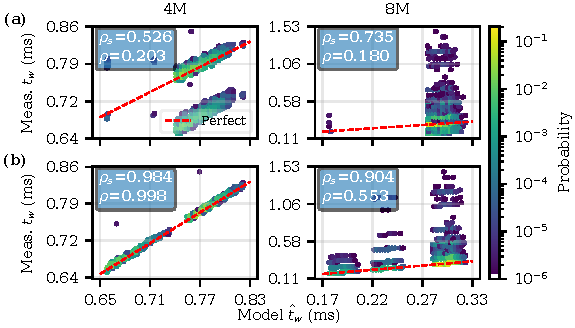
\includegraphics[width=\linewidth]{fig/images/pdf/model-comparison-codeword-vs-data.pdf}
    \vspace{-.75cm}
    \caption{Comparison of na\"ive dataword (a) and proposed codeword (b) timing models for 4M and 8M memories. Each point is colored according to the log probability that a measured $t_w$ occurs given a modeled $\hat{t}_w$.}
    % \vspace{-.2cm}
    \label{fig:timing-model}
\end{figure}

A fresh set of test vectors are generated for all 4M and 8M samples using Alg. \ref{alg:ruw}. For the na\"ive model ($d_0$,$d_1$) transitions from this test set are used directly to compute corresponding DHDs and lookup timing estimates. For our proposed model, $G_{4M}$ and $G_{8M}$ are used to produce codewords and the corresponding codeword DHDs are used to lookup timing estimates.

The test-vectors are then applied to each chip and the raw $t_{w}$ is captured (no aggregate statistics are taken). The ability of the proposed (BREW-RC-generated) timing model to predict the observed $t_{w}$ is compared to the na\"ive timing model in Figure \ref{fig:timing-model}. Both Spearman and Pearson correlation are shown as both are useful for side-channel analysis \cite{batina2008comparative}. On both chips the proposed timing model outperforms the na\"ive model. The proposed model explains almost all 4M $t_w$ variance, while rare long-tailed $t_w$ measurements present in the 8M limit improvements. These results demonstrate that the extracted parity submatrix yields a more accurate DHD, which improves timing leakage models.

% allowing for improved timing models that are critical to leakage modeling and security primitive design \cite{tolga2024trng, suri2018high}.

% Finally, we apply the test-vectors and generate $t_{wmin}$ cluster assignments ($\ell_{cw-meas}$) from the measured write latencies. We compare the ability of the BREW-RC-generated parity matrix to predict the observed $t_{ws}$ cluster with a na\"ive assignment from the data label $\ell_d$ in Figure \ref{fig:test-ruw}. The extracted parity matrices perfectly predict the cluster assignments for all applied validation $t_{ws}$ measurements. This result demonstrates that the parity matrix  
\ssection{Related Work}
\label{sec:prior}

Several studies have investigated timing side-channels in ReRAM crossbars \cite{kommareddy2019crossbar, khan2021comprehensive, krautter2022data, wang2023side}. These attacks have been evaluated by simulating these asymmetries and demonstrating how they project into various crossbar architectures. Prior investigations do not consider the effects of ECC and how ECC functions may impact crossbar timing measurements. Our results demonstrate the ECC significantly effects the timing of commercial ReRAM crossbar memories. BREW-RC closes this gap by providing a mechanism to derive timing models which incorporate timing perturbations caused by parity bit transitions.

% In this work, we will demonstrate that knowledge of codeword transition DHW $\left( w_{0\to1}, w_{1\to0} \right)$ can accurately predict the distribution of write latencies in commercial memories. However, absent knowledge of the underlying ECC function, the codeword $\left( w_{0\to1}, w_{1\to0} \right)$ becomes ambiguous, complicating timing side-channel attacks. BREW-RC (Section \ref{sec:brew-rc}) closes this gap by extracting the relationship between data bits and parity bits ($P$), allowing both the recovery of critical reliability information, and the generation of more accurate timing models in commercial ReRAM products.

% The AFM paper has no discrepencies with our work. The AFM thesis does. It'll be shorter and easier to just say we are in agreement with their work.
In \cite{tay2023investigation}, atomic force microscopy (AFM) is used to reverse engineer the logical to physical data mapping of the 4M. 
The authors de-layer the device, apply text vectors through the SPI interface, and probe the chip to determine the physical destination of the applied test vectors. 
% Assuming the presence of an ECC function, the minimum hamming distance $D_{min}$ between the reported codewords is 2, an unrealistically low $D_{min}$ for a code rate of $\frac{5}{21}$, as it provides no more error correction than a simple parity check, which can be achieved with a single bit per-word. To check our results against \cite{tay2023investigation}, 
We generate parity bits for the same set of test patterns using $G_{4M}$. We cannot know the correct physical mapping of our extracted parity bits (i.e. the column order of $P$) nor if data was loaded MSB- or LSB-first. Therefore, we compute the minimum distance between our 55 generated parity bits and the 55 parity bits reported in \cite{tay2023investigation} for all possible ($5! * 2$) arrangements and bit orders. 
% % The actual publication drops this specific set of test vectors, so I don't add it into the paper.
%   Our results have no inconsistency with the published paper, only 1 codeword in the published thesis.
\begin{figure}[t!]
    \centering
    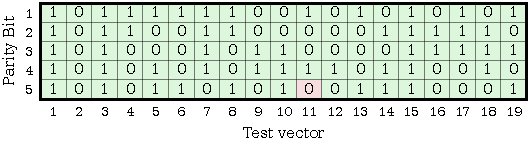
\includegraphics{fig/images/pdf/afm-comparison.pdf}
    \caption{Discrepancy between BREW-RC output and codewords reported in  \cite{tay2023thesisinvestigation}.
    \Description{An 8$\times$21 grid is shown representing the sub-array states of the MB85AS4MT under various test vectors reported in \cite{tay2023thesisinvestigation}. Green grid elements represent consistency with our results. In one location there is an inconsistency.}
    \label{fig:afm-comp}}
\end{figure}
One configuration results in a perfect match between generated codewords and the 55 parity bits reported by the authors, while the next-best configuration has a distance of 18 bits, demonstrating agreement with destructive reverse engineering techniques.
% By fixing this discrepancy, corresponding to test pattern 4, row 8 applied in \cite{tay2023investigation} (see Figure \ref{fig:afm-comp}), all codewords reported by the authors yields a reasonable $D_{min}$ for a rate $\frac{5}{21}$ ECC. We therefore believe this discrepancy to be the result of a transcription or measurement error.

\cite{tolga2024trng} and \cite{suri2018high} use the 4M to implement security primitives. Both papers use $t_w$ as an entropy source. The authors of \cite{tolga2024trng} are able to identify the a latent structure present in $t_w$ measurements but do not identify ECC as the root cause. Instead the authors truncate timing measurements, using the LSB of latency measurements to construct their proposed TRNG. The authors of \cite{suri2018high} initially observe poor PUF performance which is alleviated by effectively hashing two latency measurements using a sum-of-squares technique. Our results indicate that a significant portion of the apparent entropy in 4M/8M latency is structured by hidden ECC activity. Particularly in the 4M, knowledge of the underlying ECC explains nearly all measurement variance. We believe BREW-RC's improved timing model may be useful for improving entropy harvesting by isolating true timing variations from deterministic ECC perturbations.

% The authors note that the MB85AS4MT remains biased under their applied test patterns. Based on our analysis, we attribute this bias to hidden parity bit coupling within the devices on-chip ECC, and we believe a stronger TRNG could be realized by accounting for the full codeword structure and parity dependencies.
% Not really relavant here, this paper has so many
% In \cite{ferdaus2024hiding}, the authors implement a steganographic method to efficiently encode and decode information using the wear-level of bit-cells within the MB85AS4MT. In the context of ECC parity bit coupling, more discrete information encoding techniques may be possible in which the wear-level of ECC bits can be used rather than data bits themselves. Rather than directly hammering repeated patterns (a practice which is easily detectable in modern systems) 
\ssection{Conclusion}
In this work we presented BREW-RC, a technique to reverse engineer parity matrices from ReRAM crossbars using a novel timing side-channel. We demonstrated BREW-RC on two commercial ReRAM devices, successfully recovering the complete parity submatrix from each. We demonstrated that knowledge of ECC parity bit switching behavior substantially improves timing models. BREW-RC strengthens security analysis of ReRAM crossbar timing behavior, and provides a mechanism fo future reliability studies of commercial ReRAMs to incorporate essential ECC context.
% \input{sec/i-acknowledgements}
%%
%% The acknowledgments section is defined using the "acks" environment
%% (and NOT an unnumbered section). This ensures the proper
%% identification of the section in the article metadata, and the
%% consistent spelling of the heading.
\begin{acks}
This material is based upon work supported by the National Science Foundation under Award No. 2418268.
\end{acks}

%%
%% The next two lines define the bibliography style to be used, and
%% the bibliography file.
\clearpage
\bibliographystyle{ACM-Reference-Format}
\bibliography{
  bib/ecc,
  bib/rram_cim,
  bib/rram_crossbars,
  bib/rram_devices_overview,
  bib/rram_ecc,
  bib/rram_rad_hard,
  bib/rram_re,
  bib/rram_sec_and_sec_apps,
  bib/rram_commercial,
  bib/rram_neuromorphic,
  bib/rram_write_verify,
  bib/rram_wear
}

\end{document}
